% vim: spelllang=es

% Instrucciones:
% https://eina.unizar.es/sites/eina.unizar.es/files/archivos/secretaria/20210706_instrucciones_tfg_tfm.pdf
%
% TFGs previos:
% https://zaguan.unizar.es/search?ln=en&cc=trabajos-fin-grado&sc=1&p=inform%C3%A1tica&f=Departamento&action_search=Search
%
% Blog:
% https://nullderef.com/series/rust-plugins/
%
% NOTES:
% * Count words with `:TexWordCount`
% * Svg to pdf: `inkscape -D image.svg  -o image.pdf --export-latex`
%
% TODO:
% * Buscar typos (grep):
%   - Comas antes de conjunciones (y, e, o, u)
%   - 'Artifacto'
%   - Eliminar e.g. y i.e.
%   - Eliminar misusos de `así como`
%
% * Debería tener palabras anglosajonas con `\emph` siempre?
%
% * No sé cómo traducir onramp, offramp, sink y source de forma precisa.
%
% * Debería traducir runtime por ejecutor?
%
% * Debería incluir las figuras siempre en su sitio, donde las pone LaTeX por
% defecto, o al final de la sección?
%
% * "Figura" va en mayúsculas?

\documentclass[a4paper,12pt,twoside,hidelinks,openright]{book}

% \usepackage[T1]{fontenc}
\usepackage[spanish]{babel}
\usepackage[utf8]{inputenc}

\usepackage[usenames, dvipsnames]{color}
\usepackage{graphicx}
\usepackage{rotating}
\usepackage{multirow}
\usepackage{graphics}
\usepackage{appendix}
\usepackage[nottoc,numbib]{tocbibind}
\usepackage{xspace}

\usepackage{tikz}
\usetikzlibrary{shapes,arrows}
\usepackage{subcaption}
\usepackage{amsmath,amsthm,amssymb,mathrsfs} 
\usepackage[final]{pdfpages}
\usepackage[]{placeins,flafter}
\usepackage[none]{hyphenat} \sloppy
\usepackage{xcolor}
\usepackage{adjustbox}
\usepackage{hyperref}

% Better table formatting
\usepackage{longtable} % Multi-page tables
\renewcommand*{\arraystretch}{1.5}
\usepackage{array} % Better alignment
\newcolumntype{P}[1]{>{\centering\arraybackslash}p{#1}}
\newcolumntype{M}[1]{>{\arraybackslash}m{#1}}

% Bibtex for the bibliography
\usepackage[
    backend=bibtex,
    block=space,
    language=spanish,
    sorting=none % Sort by appearance in the document
]{biblatex}
\bibliography{Bibliografia_TFG}

% Easier to read font
\usepackage{fourier} % For math
\usepackage{fontspec}
\setmainfont{Heuristica} % For the text
\setmonofont{Liberation Mono} % For the code

% Less margin between lists, otherwise after overriding \parskip and etc it's
% too much.
\usepackage{enumitem}
\setlist{topsep=0pt}

% Code syntax highlighting. The cache is hardcoded with an absolute path for the
% Tectonic engine until this is fixed:
% https://github.com/tectonic-typesetting/tectonic/issues/835
\usepackage[
    cachedir=/home/mario/Downloads/minted/
]{minted}
\usepackage{xcolor}
\usemintedstyle{friendly}
\definecolor{bg}{HTML}{f8f8f8}
\setminted{
    frame=lines,
    framesep=2mm,
    bgcolor=bg,
    fontsize=\footnotesize,
    linenos
}

% Remove red boxes around illegal characters in minted, taken from:
% https://tex.stackexchange.com/a/343506
%
% This way, `mysql` can be used to highlight tremorscript as a quick hack.
\makeatletter
\AtBeginEnvironment{minted}{\dontdofcolorbox}
\def\dontdofcolorbox{\renewcommand\fcolorbox[4][]{##4}}
\makeatother

% Command for inline code
\newmintinline[code]{text}{fontsize=\normalsize}
\newmintinline[rust]{rust}{fontsize=\normalsize}
\newcommand{\image}[1] {
  \begin{figure}[H]
    \centering
    \includegraphics[width=\textwidth]{#1}
  \end{figure}
}
% Shortcuts
\newcommand{\cpp}{C\texttt{++}}
\newcommand{\cratelink}[1] {%
    \code{#1}\footnote{\url{https://crates.io/crates/#1}}\xspace%
}
\newcommand{\work}{``Primero haz que Funcione''\xspace}
\newcommand{\unsafe}{\code{unsafe}\xspace}
\newcommand{\abistable}{\code{abi_stable}\xspace}
% Gracias unizar por no evolucionar y solo permitir memorias en castellano...
\newcommand{\crate}{\emph{crate}\xspace}
\newcommand{\crates}{\emph{crates}\xspace}
\newcommand{\onramp}{\emph{onramp}\xspace}
\newcommand{\onramps}{\emph{onramps}\xspace}
\newcommand{\offramp}{\emph{offramp}\xspace}
\newcommand{\offramps}{\emph{offramps}\xspace}
\newcommand{\sink}{\emph{sink}\xspace}
\newcommand{\sinks}{\emph{sinks}\xspace}
\newcommand{\source}{\emph{source}\xspace}
\newcommand{\sources}{\emph{sources}\xspace}
\newcommand{\pipeline}{\emph{pipeline}\xspace}
\newcommand{\pipelines}{\emph{pipelines}\xspace}
\newcommand{\builder}{\emph{builder}\xspace}
\newcommand{\builders}{\emph{builders}\xspace}
\newcommand{\lifetime}{\emph{lifetime}\xspace}
\newcommand{\lifetimes}{\emph{lifetimes}\xspace}
\newcommand{\websockets}{\emph{websockets}\xspace}
\newcommand{\trait}{\emph{trait}\xspace}
\newcommand{\traits}{\emph{traits}\xspace}
\newcommand{\struct}{\emph{struct}\xspace}
\newcommand{\structs}{\emph{structs}\xspace}
\newcommand{\leak}{\emph{leak}\xspace}
\newcommand{\leaks}{\emph{leaks}\xspace}
\newcommand{\scripting}{\emph{scripting}\xspace}
\newcommand{\sandbox}{\emph{sandbox}\xspace}
\newcommand{\sandboxing}{\emph{sandboxing}\xspace}
\newcommand{\socket}{\emph{socket}\xspace}
\newcommand{\sockets}{\emph{sockets}\xspace}
\newcommand{\stdin}{\emph{stdin}\xspace}
\newcommand{\stdout}{\emph{stdout}\xspace}
\newcommand{\stderr}{\emph{stderr}\xspace}
\newcommand{\csharp}{C\#\xspace}
\newcommand{\pipe}{\emph{pipe}\xspace}
\newcommand{\pipes}{\emph{pipes}\xspace}

%	CONFIGURACIÓN DE PÁGINA

\setlength{\paperwidth}{21cm}          % Ancho de página
\setlength{\paperheight}{29,7cm}       % Alto de página
\setlength{\textwidth}{15.5cm}         % Ancho de zona con texto
\setlength{\textheight}{24.6cm}        % Ancho de zona con texto
\setlength{\topmargin}{-1.0cm}         % Margen superior
                                      
\setlength{\oddsidemargin}{0.46cm}     % Margen izquierdo 
\setlength{\evensidemargin}{0.46cm}    

\usepackage{makeidx}
\makeindex
\index{key}
\newcommand{\myref}[1]{\color{red}\bf(\ref{#1})}


\begin{document}

% PORTADA
\begin{titlepage}

\definecolor{unizarblue}{RGB}{0, 86, 153}

\vspace*{-4mm}
\begin{figure}[!h]
  \centering
	
\includegraphics[width=69.62mm]{Imagenes/UnizarLogo}
\end{figure}

\vspace*{17mm}

\fontsize{28pt}{28pt}\selectfont
\begin{center}
\setlength{\fboxsep}{3.4mm}
\adjustbox{minipage=14.4cm,cfbox=unizarblue,center}{\begin{center} Trabajo Fin de Grado \end{center}}
\end{center}

\vspace*{18.7mm}

\fontsize{22pt}{22pt}\selectfont
\begin{center}
\textsc{Cargado dinámico de plugins en Rust\\
en ausencia de estabilidad en la\\
Interfaz Binaria de Aplicación}
\end{center}

\vspace*{0.75cm} 

\fontsize{22pt}{22pt}\selectfont
\begin{center}
\textsc{Dynamic loading of plugins in Rust \\
in the absence of a stable \\
Application Binary Interface}
\end{center}

\vspace*{2cm} 
\baselineskip 36pt
\begin{center}

\fontsize{14pt}{14pt}\selectfont
\center{\rm Autor:}
\vspace*{0mm} 
\fontsize{18pt}{18pt}\selectfont
\center{\textsc{Mario Ortiz Manero}}

\baselineskip 36pt

\fontsize{14pt}{14pt}\selectfont
\center{\rm  Director:}
\vspace*{0mm}
\fontsize{15pt}{15pt}\selectfont
\center{\textsc{Javier Fabra Caro}}

\end{center}

\setcounter{footnote}{1}

\vspace*{2cm}
\fontsize{14pt}{14pt}\selectfont
\begin{center}
Grado en Ingeniería Informática\\ \medskip
Departamento de Ingeniería e Ingeniería de Sistemas\\
Escuela de Ingeniería y Arquitectura\\ \bigskip
Junio 2022\\
\end{center}


\renewcommand{\thefootnote}{\arabic{footnote}}
\pagenumbering{gobble}
\end{titlepage}
\newpage


\title{Dynamic loading of plugins in Rust in the absence of a stable Application Binary Interface}
\author{Mario Ortiz Manero}

\pagebreak
\cleardoublepage%
\baselineskip 19pt

\renewcommand{\labelitemi}{$-$}
\renewcommand{\tablename}{Tabla}

\renewcommand{\appendixname}{Anexos}
\renewcommand{\appendixtocname}{Anexos}
\renewcommand{\appendixpagename}{Anexos}


\pagenumbering{Roman}

% Párrafos de forma más convencional, me parece más fácil leerlo así.
\begingroup
\setlength{\parskip}{\baselineskip}%
\setlength{\parindent}{0pt}%

\newpage
\cleardoublepage%
% vim: spelllang=es

\begin{center}
{\LARGE \bfseries AGRADECIMIENTOS}
\vspace{2.5cm}
\end{center}

Un primer gracias a toda mi familia por apoyarme en cualquier momento que lo
necesitara. En especial, a mi padre y a mi madre por aguantarme siempre y por
dejarse la piel para que pueda estudiar.

A mis amigos que me han acompañado toda la vida con tan buenos momentos, y a los
de la universidad, que fueron la verdadera motivación a ir a clase y seguir día
a día. Las horas incontables juntos en la biblioteca, en el bar de la EINA o
incluso en los montes más recónditos de Juslibol a las dos de la madrugada, han
hecho que estos años merezcan la pena.

También a mis profesores por orientarme, particularmente a Javier Fabra por
ayudarme con mi Erasmus, este documento y todas sus complicaciones. Mis mentores
de Tremor tomaron un papel fundamental, no solo dándome consejo para el
proyecto, sino también para mi carrera profesional y mi vida.

Finalmente, agradecer a todas las organizaciones que han hecho esto posible. A
la Fundación de Linux por ofrecer los medios. A Wayfair por apostar sus fondos
en código abierto y talento joven. Y a la comunidad de código abierto, que me ha
motivado a programar desde el principio y me ha guiado hasta donde estoy hoy.


\newpage
\cleardoublepage%
% vim: spelllang=es

\begin{center}
{\LARGE \bfseries RESUMEN}

\vspace{2.5cm}
\end{center}

La toma de decisiones de muchas empresas modernas como Wayfair se basa en la
recolección y análisis de datos de sus sistemas. Para llevarlo a cabo de forma
eficiente en una escala masiva, es necesario el uso de herramientas de alto
rendimiento como Tremor, escrito con Rust, programación asíncrona y SIMD.

A medida que Tremor evoluciona, sus tiempos de compilación crecen y,
consecuentemente, se deteriora la experiencia de desarrollo. Esto se puede
aliviar implementando un sistema de plugins que divide su único binario en
componentes más pequeños compilables independientemente.

Existen múltiples tecnologías disponibles para su desarrollo: lenguajes
interpretados, WebAssembly, eBPF, comunicación inter-proceso o cargado dinámico.
Sin embargo, gran parte de ellas deben descartarse por no cumplir los estándares
de eficiencia de Tremor. Entre las alternativas restantes, se escoge cargado
dinámico por ser la más usable y popular.

El cargado dinámico es imposible con tipos y funciones declarados con Rust puro,
ya que su Interfaz Binaria de Aplicación (ABI) no es estable. Será necesario
convertir los tipos al ABI de C, que sí es estable, y viceversa. Para facilitar
el proceso, se pueden aprovechar librerías existentes y herramientas del
lenguaje como macros procedurales.

Dado que el cargado dinámico en Rust es un ecosistema muy nuevo, es necesario
contribuir en código abierto a gran cantidad de sus dependencias para
implementar la funcionalidad necesaria para un sistema de plugins.

La complejidad del proyecto incrementó significativamente respecto al plan
original, por lo que aunque funcional, no alcanza alguno de los objetivos
iniciales, principalmente relacionados con el rendimiento. Sin embargo, sirve
como una buena base para futuras versiones de Tremor que sí que lo incluyan en
producción, y continuará evolucionando con el programa.


\newpage
\cleardoublepage%
% vim: spelllang=en

\begin{center}
{\LARGE \bfseries ABSTRACT}

\vspace{2.5cm}
\end{center}


Una mañana, tras un sueño intranquilo, Gregorio Samsa se despertó convertido en un monstruoso insecto. Estaba echado de espaldas sobre un duro caparazón y, al alzar la cabeza, vio su vientre convexo y oscuro, surcado por curvadas callosidades, sobre el que casi no se aguantaba la colcha, que estaba a punto de escurrirse hasta el suelo. Numerosas patas, penosamente delgadas en comparación con el grosor normal de sus piernas, se agitaban sin concierto. - ¿Qué me ha ocurrido? No estaba soñando. Su habitación, una habitación normal, aunque muy pequeña, tenía el aspecto habitual. Sobre la mesa había desparramado un muestrario de paños - Samsa era viajante de comercio-, y de la pared colgaba una estampa recientemente recortada de una revista ilustrada y puesta en un marco dorado. La estampa mostraba a una mujer tocada con un gorro de pieles, envuelta en una estola también de pieles, y que, muy erguida, esgrimía un amplio manguito, asimismo de piel, que ocultaba todo su antebrazo. Gregorio miró hacia la ventana; estaba nublado, y sobre el cinc del alféizar repiqueteaban las gotas de lluvia, lo que le hizo sentir una gran melancolía. «Bueno -pensó-; ¿y si siguiese durmiendo un rato y me olvidase de

\endgroup

\newpage
\cleardoublepage%
\renewcommand{\contentsname}{Índice}
\tableofcontents

\newpage
\renewcommand\listfigurename{Lista de Figuras}
\listoffigures

\newpage
\renewcommand\listtablename{Lista de Tablas}
\listoftables

TODO: quito la lista de tablas? Lo único que hay es del anexo.

% Capitulos

% Vuelta a configurar los párrafos para que no afecte al índice
\begingroup
\setlength{\parskip}{\baselineskip}%
\setlength{\parindent}{0pt}%

% vim: spelllang=es

\chapter{Introducción}
\pagenumbering{arabic}

\section{Contexto}

% TODO: quizá algunos footnotes podrían cambiarse por referencias aquí
Este proyecto se ha realizado en colaboración con
\emph{Tremor}\footnote{\url{https://tremor.rs}}, un sistema de procesado de
eventos de alto rendimiento, escrito en el lenguaje de programación
\emph{Rust}\footnote{\url{https://www.rust-lang.org}}. Tremor es un programa de
código abierto bajo la fundación \emph{Cloud Native Computing
Foundation~(CNCF)}\footnote{\url{https://www.cncf.io/}}, que es también parte de
la organización \emph{Linux
Foundation~(LFX)}\footnote{\url{https://www.linuxfoundation.org/}}.

Formalmente, el trabajo se ha llevado a cabo gracias a la iniciativa \emph{LFX
Mentorship}, con el título ``CNCF -- Tremor: Add plugin support for tremor
(PDK)''\footnote{Página oficial de la iniciativa:
\url{https://mentorship.lfx.linuxfoundation.org/project/b90f7174-fc53-40bc-b9e2-9905f88c38ff}}\footnote{\emph{Tracking
issue} en GitHub:
\url{https://github.com/tremor-rs/tremor-runtime/issues/791}}\footnote{RFC en la
documentación de Tremor:
\url{https://www.tremor.rs/rfc/accepted/plugin-development-kit/}}. Esta
iniciativa promueve el aprendizaje de desarrolladores de código abierto,
proporcionando una plataforma transparente y facilitando un sistema de pagos.

Finalmente, \emph{Wayfair} es una empresa estadounidense de comercio digital de
muebles y artículos del hogar\footnote{\url{https://www.wayfair.com/}}.
Actualmente, ofrece 14 millones de ítems de más de 11.000 proveedores
globales~\cite{wayfairItems} y es el principal financiador tanto de Tremor como
de este proyecto.

\section{Objetivo}

La tarea a llevar a cabo es la implementación de un sistema de plugins,
denominado \emph{Plugin Development Kit~(PDK)}, para la base de código ya
existente en Tremor.

Esto es una tarea no-trivial, dado que Rust no tiene un \emph{Application Binary
Interface~(ABI)} estable. Es decir, que si se compila la \emph{runtime} (el
binario principal encargado de cargar funcionalidad externa) y los
\emph{plugins} (los binarios individuales con la funcionalidad) de forma
separada, no hay garantía de que la representación binaria de los datos o la
convención de llamada a funciones --- entre otros --- sea la misma.

Esto implica que \emph{dynamic loading} es imposible de forma segura puramente
con Rust, debiéndose recurrir a otro ABI que sí sea estable, como el del
lenguaje de programación C. Por tanto, se deben escribir \emph{bindings} (la
definición de la interfaz compartida entre runtime y plugins) completas en C y
transformar tipos de Rust a C y viceversa cuando se interactúe con plugins.

\section{Motivación}

\subsection{Tiempos de compilación}

% TODO: incluir modo release?
Actualmente, el problema más importante en Tremor es sus tiempos de compilación.
En un ordenador de gama media de \~{}600 € como el Dell Vostro 5481, compilar el
binario \code{tremor} desde cero requiere de más de 7 minutos en modo debug.
Incluso en el caso de cambios incrementales (una vez las dependencias ya han
sido compiladas), hay que esperar unos 10 segundos. Esto no es una buena
experiencia de desarrollo e impide que nuevos programadores se unan a la
comunidad de Tremor.

Debido a la naturaleza del programa, este problema solo empeorará con el tiempo.
Tremor debe tener soporte para un gran número de protocolos (e.g., TCP o UDP),
software (e.g., Kafka o PostgreSQL) y codecs (e.g., JSON o YAML). El número de
dependencias continuará incrementando hasta que imposibilite la creación de
nuevas prestaciones en Tremor.

Los problemas relacionados con tiempos de compilación excesivamente largos no se
limitan a Tremor. Es uno de las mayores críticas que recibe Rust y un 61\% de
sus usuarios declaran que aún se necesita trabajo para mejorar la
situación~\cite{rustsurvey}.

\subsection{Modularidad}

Otra ventaja que provee un sistema de plugins es modularidad; ser capaz de
tratar la runtime y los plugins de forma separada suele resultar en una
arquitectura más limpia~\cite{baldwin2000design}. También hace posible el
desacoplamiento del ejecutable y sus componentes; algunas dependencias tienen un
ciclo de versionado más rápido que otras y generalmente es más conveniente
actualizar únicamente un plugin, en lugar del programa por completo.

\subsection{Aprender de otros}

Otros proyectos maduros con características similares a las de Tremor, como
\textcite{nginx} o \textcite{apachehttpserver}, llevan beneficiándose de un
sistema de plugins desde hace mucho. Informan mejorías en flexibilidad,
extensibilidad y facilidad de
desarrollo~\cite{nginxPluginsAdvantages}\cite{apachePluginsAdvantages}. Aunque
las desventajas también mencionen un pequeño impacto en el rendimiento y la
posibilidad de caer en un \emph{dependency hell}, sigue siendo una buena idea al
menos considerarlo para Tremor.

\section{Metodología}

\subsection{Organización}

El proyecto ha tenido una duración de unos 10 meses, comenzando en agosto de
2021 y terminando en mayo/junio de 2022. Su realización ha sido completamente
remota y con horarios muy flexibles. Se usó el servidor de Discord de
Tremor\footnote{\url{https://discord.com/invite/Wjqu5H9rhQ}} como plataforma
principal para comunicarse, tanto por texto como por videollamada. Se programó
una llamada por semana, en la que explicaba mi progreso y recibía ayuda de mis
mentores en caso de que me hubiera quedado atascado en algún momento.

% TODO: update Matthias' title
Disponía de tres mentores, que me guiaban en el proceso de desarrollo: Darach
Ennis (\emph{Principal Engineer and Director of Tremor Project}), Matthias Wahl
(\emph{Staff Engineer}) y Heinz N. Gies (\emph{Senior Staff Engineer}), todos
empleados por Wayfair.

La organización de forma más estructurada para las tareas que tenía pendientes,
en las que estaba trabajando en ese momento, y las que ya había realizado, se
basó principalmente en un Kanban en
GitHub\footnote{\url{https://github.com/marioortizmanero/tremor-runtime/projects/1}}.

\subsection{Desarrollo}

Para reducir el coste de desarrollo y asegurarse de que el proceso sea
completamente seguro (en memoria y concurrencia), el sistema de plugins
aprovecha librerías existentes en Rust y herramientas como macros procedurales.
El sistema de compilación usado es solución oficial de Rust: Cargo, que también
incluye un \emph{formatter}, \emph{linter}, y extensiones instalables creadas
por la comunidad. Adicionalmente, existe una gran cantidad de tests y
\emph{benchmarks} que se han de tener en cuenta para mantener el \emph{Code
Coverage} (la cantidad de código cubierta por los tests) y el rendimiento.

\subsection{Recursos públicos}

% TODO: actualizar '5' cuando suba el nuevo
% TODO: actualizar minutos de lectura
% TODO: al terminar, mencionar qué no se incluye aquí de los blogs
% TODO: buscar otra métrica que no sean horas de lectura, no creo que sea buena
% manera de venderlo
Este trabajo está disponible públicamente al completo. Además, a medida que he
investigado e implementado el sistema de plugins, he ido escribiendo todo en mi
blog personal, \emph{NullDeref}; gran parte de los contenidos de este documento
se han obtenido de ahí. Tiene una serie con un total de 5 artículos que entran
en gran detalle y suman unas 2 horas adicionales de lectura.

\begin{itemize}
    \item El repositorio de GitHub para el binario de Tremor:\\
        \url{https://github.com/tremor-rs/tremor-runtime}
    \item Mi \emph{fork}, con ramas adicionales usadas durante el desarrollo:\\
        \url{https://github.com/marioortizmanero/tremor-runtime}
    \item Mi repositorio con experimentos antes de implementar la versión
        definitiva:\\
        \url{https://github.com/marioortizmanero/pdk-experiments}
    \item La serie de artículos en mi blog personal:\\
        \url{https://nullderef.com/series/rust-plugins/}.
\end{itemize}

TODO: debería ser más específico sobre las horas? Mucha cuenta no he llevado
pero vamos sí que estoy segurísimo de que han sido 300 horas y mucho más
también.

TODO: debería incluir que atendí a KubeCon 2022 gracias a Tremor, explicándolo
un poco en un anexo?

TODO: quizá hacer una tabla que relacione cada sección del índice con los
capítulos relacionados de nullderef? Pero eso ya lo pondría en un anexo.

% vim: spelllang=es

\chapter{Breve introducción a Rust}\label{ch:rust}

Dado que Rust es un lenguaje de programación que tan solo anunció su primera
versión en 2015, aún no es conocido por muchos desarrolladores. Este proyecto
requiere ser familiar con cómo funciona, por lo que en este capítulo se
introducirán los conceptos más básicos necesarios. Sí que se asume conocimiento
de lenguajes de propósito general, como C, C++, Python o Java.

Sin embargo, es posible que se omitan algunos conceptos o que algunas
explicaciones no sean completamente precisas por razones de simplicidad.
\textcite{rustfullbook} es el libro oficial para aprender Rust por completo,
pero es una lectura larga y posiblemente demasiado exhaustiva. Para mayor
brevedad, se recomienda leer \textcite{rustprofessionals},
\textcite{rustgentleintro} o \textcite{rust30min}.

La comunidad dispone de otros libros que explican aspectos más avanzados del
lenguaje en específico, como \unsafe o la programación asíncrona. En esos casos,
se recomienda leer \textcite{rustnomicon} y \textcite{rustasyncbook},
respectivamente.

TODO: revisar traducciones del libro o similares para asegurarse de que la
terminología es la misma.

\section{¿Qué es Rust?}

Rust es un lenguaje de programación de sistemas compilado y de propósito
general. Su objetivo es maximizar rendimiento y usabilidad, esto último
basándose en seguridad integrada en el lenguaje, en vez de en el \

\section{Primeros pasos}

Comenzando por el clásico ``Hola Mundo'', se incluyen algunos ejemplos de cómo
es la sintaxis de Rust más básica. El programa se podría ejecutar fácilmente con
\emph{Cargo}, el administrador de dependencias oficial, o específicamente con el
comando \code{cargo run}.

\begin{minted}{rust}
fn main() {
    println!("Hello World!");
}
\end{minted}

\code{main} es nuestra función principal, que invoca al macro \emph{println}
para escribir por pantalla. Esto se sabe porque, a diferencia de una llamada a
función, la invocación termina con una exclamación (\code{!}).

Los bloques básicos (\code{if}, \code{else}, \code{while}, \code{for}) son los
mismos que en otros lenguajes, con la introducción de \code{match}, que permite
extraer patrones.

\begin{minted}{rust}
fn factorial(i: u64) -> u64 {
    match i {
        0 => 1,
        n => n * factorial(n-1)
    }
}
\end{minted}

\section{Librería estándar}

De forma similar a C++, Rust posee tipos genéricos. Esto permite la
implementación de una librería estándar flexible, con varias estructuras de
datos importantes a conocer:

\begin{itemize}
    \item Tipos primitivos:
        \begin{itemize}
            \item Carácteres con \code{char}.

            \item Punto flotante con \code{f32} y \code{f64}.

            \item Booleanos con \code{bool}.

            \item Enteros: \code{u8}, \code{i8}, \code{u16}, \code{i16},
                \code{u32}, \code{i32}, \code{u64}, \code{i64}, e incluso
                \code{i128} y \code{u128} en las arquitecturas que lo soportan.

            \item Vectores de tamaño fijo: por ejemplo \code{[1, 2, 3, 4, 5]}.

            \item N-tuplas como \code{(1, true, 9.2)}.

            \item El tipo ``unidad'', \code{()}, equivalente a \code{void} en C
                o C++.

            \item Punteros básicos con \code{*const T} o \code{*mut T}.

        \end{itemize}

    \item \code{Vec<T>} representa un vector contiguo y redimensionable.

    \item \code{HashMap<K, V>} es una tabla hash, genérica respecto a su clave
        \code{K} y su valor \code{V}. No se encuentra en el preludio, por lo que
        requeriría la siguiente declaración, similar a un \code{import} de Java:

\begin{minted}{rust}
use std::collections::HashMap;
\end{minted}

    \item \code{Box<T>}, usado para localizar un tipo \code{T} en memoria.
        Incluye el tamaño que ocupa \code{T}.

    \item \code{str} es una cadena UTF-8 de solo lectura, típicamente usada con
        una referencia \code{&str}. Va acompañada por su longitud, por lo que no
        hace falta terminarla con \code{\0}, a diferencia de C. \code{String} es
        su versión modificable asignada en memoria.

\end{itemize}

\section{Gestión de errores}

En Rust, los errores se indican con el tipo \code{Result<T, E>}. Este se trata
de una enumeración cuyo valor puede ser \code{Ok(T)}, con el resultado obtenido
satisfactoriamente, o \code{Err(E)}, con el tipo de error que ha sucedido. Dado
que es un tipo nuevo, si el programador se olvidase de comprobar errores, el
programa no compilaría. Se puede usar \code{match} para comprobar el resultado,
o una serie de funciones disponibles para hacer el proceso más ergonómico:

\begin{minted}{rust}
match load_file(input) {
    Ok(data) => /* ... */,
    Err(e) => eprintln!("Error: {e}"),
}
\end{minted}

En caso de que se produjera un error del que el programa no se puediera
recuperar, como quedarse sin memoria o un fallo inesperado en la implementación,
se usa la funcionalidad de \emph{pánicos}. Un pánico se propaga de forma similar
a una excepción de C++ o Java, y terminará la ejecución por completo. Esto se
puede invocar con el macro \code{panic!} o utilidades similares.

\section{Macros}

Rust da soporte para dos tipos de macros, los \emph{declarativos}, y los
\emph{procedurales}. Sin entrar en excesivo detalle, los declarativos se pueden
implementar de forma similar al caso de C o C++, como si se tratase de una
función con una sintaxis especial. Los procedurales son mucho más costosos

\begin{minted}{rust}
some_macro!(1, 2, 3); // Puede ser tanto declarativo como procedural
\end{minted}

\begin{minted}{rust}
// Con macros declarativos
some_macro! {
    fn some_function() { /* ... */ }
}

// Con macros procedurales
#[some_macro]
fn some_function() { /* ... */ }
\end{minted}

\begin{minted}{rust}
// Los de tipo `derive` son solo posibles con EEEEPAAAA
\end{minted}

% vim: spelllang=es

\chapter{Entendiendo Tremor}\label{ch:tremor}

\section{Procesado de Eventos}

Tremor es un \emph{Sistema de Procesado de Eventos}, que consiste en ``el
monitorizado y análisis (procesado) de flujos de información (datos) sobre cosas
que pasan (eventos)''~\cite{luckham2011event}. Tremor fue creado como una
alternativa de alto rendimiento a herramientas como \textcite{logstash} o
\textcite{telegraf}, pero ha evolucionado para soportar casos de uso más
complejos. Al contrario que esos programas, Tremor también tiene soporte para
\emph{agregación} y \emph{rollups}, e incluye un lenguaje \emph{ad hoc} para
\emph{Extract, Transform, and Load} (ETL).

% TODO: hace falta esto?
\textcite{robins2010complex} y \textcite{cugola2012processing} introducen en
detalle los dos campos contenidos en Procesado de Eventos: \emph{Procesado de
Eventos Complejos} y \emph{Procesado de Flujos de
Eventos}\footnote{\emph{Complex Event Processing} y \emph{Event Stream
Processing} respectivamente, siguiendo la terminología anglosajona.}, ambos
relevantes a Tremor. \textcite{dayarathna2018recent} y
\textcite{tawsif2018review} resumen los avances más recientes en el campo,
analizan su evolución, y clasifican sus subáreas. La mayoría de la información
teórica en esta sección se extrae de estas fuentes.

\section{Casos de uso}

La Figura~\ref{fig:tremor_example} ilustra uno de los casos de uso más básicos
de Tremor:

\begin{enumerate}
    \item Recibir \emph{logs} (eventos) de aplicaciones en diferentes protocolos
        o formatos. Es posible que esta heterogeneidad se deba a que algunas
        aplicaciones son legadas y no se puedan reducir a un único protocolo o
        formato, o que esta tarea es demasiado compleja como para gestionarse a
        nivel de aplicación.

    \item Filtrar los eventos redundantes, añadir campos nuevos o eliminar
        aquellos innecesarios y transformar todo a un mismo formato. El uso de
        una herramienta ineficiente o \emph{ad hoc} por la empresa podría ser
        inviable dada una cantidad de datos suficientemente grande o demasiados
        protocolos y formatos como para implementarlos todos.

    \item Enviar todos los logs estructurados a una base de datos para
        analizarlos posteriormente.

\end{enumerate}

\begin{figure}
    \centering
    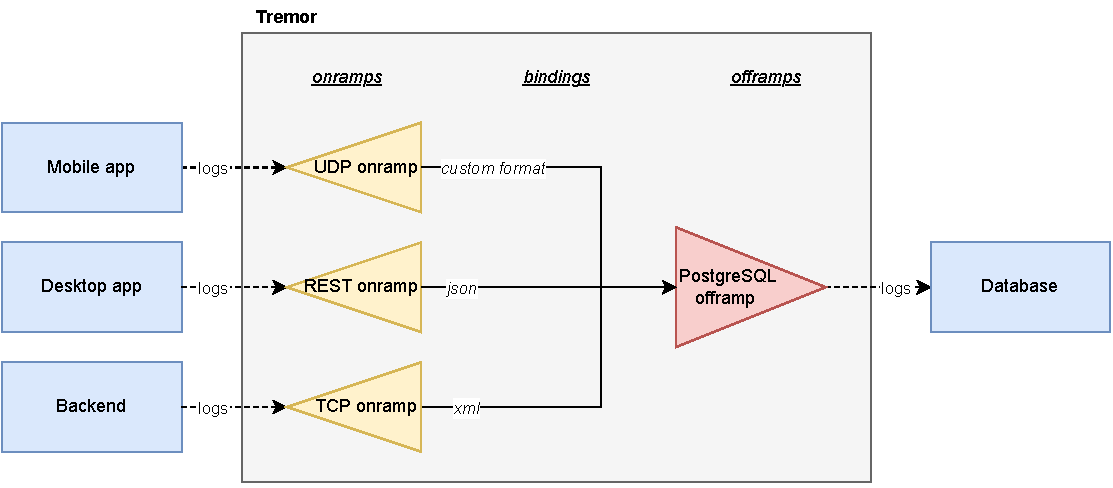
\includegraphics[width=\textwidth]{./Imagenes/example.pdf}
    \caption{Ejemplo de uso básico de Tremor}%
    \label{fig:tremor_example}
\end{figure}

Sin embargo, este caso subestima el potencial de Tremor. La entrada y salida del
sistema se pueden abstraer más, por ejemplo implementando un chatbot que
reproduce música. Este podría tomar mensajes de Discord como su entrada, y
enviar comandos con el API de Spotify como salida.

\section{Conceptos básicos}

Tremor se basa en los términos de \onramps o \sources y \offramps o \sinks:

\begin{itemize}
    \item Una \onramp especifica cómo Tremor se conecta con el mundo exterior (o
        una \pipeline) para \textbf{recibir} de sistemas externos. Por ejemplo
        TCP, periódicamente o PostgreSQL~\cite{tremoronramps}.

    \item Una \offramp especifica cómo Tremor se conecta con el mundo exterior
        (o una \pipeline) para \textbf{enviar} a sistemas externos. Por ejemplo,
        \emph{stdout}, Kafka o ElasticSearch~\cite{tremorofframps}.

    \item Una \pipeline es una lista de operaciones (transformación, agregación,
        eliminación, etc) a través de la cual se pueden encaminar los
        eventos~\cite{tremorpipelines}. La Figura \ref{fig:tremor_pipeline}
        muestra un ejemplo de una \pipeline, definida con Troy, su propio
        lenguaje inspirado en SQL.

\end{itemize}

TODO: mover lo siguiente al anexo y mencionar el leerlo para más detalles?

\begin{figure}
    \centering
    \begin{minted}[escapeinside=||]{mysql}
|\textcolor{blue}{define pipeline}| main
# The exit port is not a default port, so we have to overwrite the
# built-in port selection
into |out, exit|
|\textcolor{blue}{pipeline}|
  # Use the `std::string` module
  use std::|string|;
  use lib::scripts;

  # Create our script
  create |\textcolor{blue}{script}| punctuate from scripts::punctuate;

  # Filter any event that just is `"exit"` and send it to the exit port
  select {"graceful": false} from |in| where event == "exit" into |exit|;

  # Wire our capitailized text to the script
  select |string|::capitalize(event) from |in| where event != "exit"
    into punctuate;
  # Wire our script to the output
  select event from punctuate into |out|;
end;
    \end{minted}
    \caption{Ejemplo de una \pipeline definida para Tremor}%
    \label{fig:tremor_pipeline}
\end{figure}

Estos \onramps u \offramps suelen contener una cantidad de información que es
demasiado grande como para guardarla y debería tratarse en tiempo real. Su
procesado se basa en las siguientes operaciones:

\begin{itemize}
    \item \emph{Filtros}: descarte de eventos completos a partir de reglas
        configuradas, con el objetivo de eliminar información de la \pipeline
        que no se considera relevante.

    \item \emph{Transformaciones}: conversión de los datos de un formato a otro,
        así como incrementar un campo con un contador, reemplazar valores, o
        reorganizar su estructura.

    \item \emph{Matching}: búsqueda de partes de los eventos que siguen un
        patrón en específico (e.g., un campo \code{"id"} con un valor númerico)
        para transformarlo o descartarlo.

    \item \emph{Agregación} o \emph{rollups}: recolección de múltiples eventos
        para producir otros nuevos (e.g., la media o máximo de un campo), de
        forma que la información útil se reduzca en tamaño.

\end{itemize}

Finalmente, otros términos misceláneos sobre Tremor:

\begin{itemize}
    \item \emph{Códec}: describen cómo decodificar los datos del flujo y como
        volverlos a codificar. Por ejemplo, si los eventos de entrada usan JSON,
        tendrá que especificarse ese códec para que lo pueda entender Tremor.

    \item \emph{Preprocesador} o \emph{postprocesador}: operadores sobre flujos
        de datos brutos. Un preprocesador aplicará esta operación antes del
        códec y un postprocesador después. Por ejemplo, \code{base64} codifica o
        decodifica la información con ese protocolo.

    \item \emph{Artefacto}: término genérico para hablar de \sinks, \sources,
        códecs, preprocesadores y postprocesadores.

\end{itemize}

Para más información sobre Tremor se puede consultar \textcite{tremorintro}, que
introduce sus conceptos más básicos y sus posibles usos --- o cuándo \emph{no}
usarlo, en \textcite{tremorconstraints}. \textcite{tremorrecipes} lista un total
de 32 ejemplos de cómo configurar y emplear el software.

\section{Conectores}

Sin embargo, es posible que algunas \onramps no solo quieran recibir de sistemas
externos, sino también responderles directamente, actuando como una \offramp y
viceversa. Esto es especialmente útil para casos como REST y \websockets, donde
el protocolo da la posibilidad de responder a eventos, por ejemplo con un ACK,
usando la misma conexión. En la versión 0.11 --- la presente cuando me uní al
proyecto --- este problema se solucionaba con el concepto de \emph{linked
transports}.

El término \emph{conector} se introdujo en mayo de 2022 con la versión 0.12.
Solucionan el problema desde el inicio, abstrayendo tanto los \onramps como los
\offramps bajo el mismo concepto, incluyendo los \emph{linked transports}. Dado
que estos ya estaban siendo desarrollados mientras 0.11 era la última versión,
el sistema de plugins se enfocó a conectores desde el principio, en lugar de
\onramps u \offramps, que actualmente están en desuso.

A nivel de implementación, los conectores se definen con el \trait
\rust{Connector}, incluido en la figura \ref{fig:tremor_connector_trait}.
Esencialmente, los plugins de tipo conector exportarán públicamente esta
interfaz en su binario, y la runtime deberá ser capaz de cargarlo dinámicamente.
Actualmente, todos los conectores disponibles se listan y cargan de forma
estática al inicio del programa.

Por tanto, es importante mantener la interfaz de plugins lo más simple posible.
Los detalles de comunicación deberían dejarse a la runtime, de forma que los
plugins se limiten a exportar una lista de funciones síncronas. De esta forma,
se podrá evitar pasar tipos complejos (\rust{async}, canales de comunicación,
etc) entre la runtime y los plugins, que implicaría una carga de trabajo mucho
más alta.

Una vez esta interfaz de bajo nivel se defina, se puede crear un \emph{wrapper}
de más alto nivel en la runtime que se encargue de la comunicación y de mejorar
su usabilidad dentro de Tremor. Esto mismo lo hacen otras \crates como
\cratelink{rdkafka}, que implementa una capa de abstracción asíncrona sobre su
interfaz de C en \cratelink{rdkafka-sys}.

% vim: spelllang=es

\chapter{Validación experimental}

Lorem ipsum dolor sit amet, consectetuer adipiscing elit. Aenean commodo ligula eget dolor. Aenean massa. Cum sociis natoque penatibus et magnis dis parturient montes, nascetur ridiculus mus. Donec quam felis, ultricies nec, pellentesque eu, pretium quis, sem. Nulla consequat massa quis enim. Donec pede justo, fringilla vel, aliquet nec, vulputate eget, arcu. In enim justo, rhoncus ut, imperdiet a, venenatis vitae, justo. Nullam dictum felis eu pede mollis pretium. Integer tincidunt. Cras dapibus. Vivamus elementum semper nisi. Aenean vulputate eleifend tellus. Aenean leo ligula, porttitor eu, consequat vitae, eleifend ac, enim. Aliquam lorem ante, dapibus in, viverra quis, feugiat a, tellus. Phasellus viverra nulla ut metus varius laoreet. Quisque rutrum. Aenean imperdiet. Etiam ultricies nisi vel augue. Curabitur ullamcorper ultricies nisi. Nam eget dui. Etiam rhoncus. Maecenas tempus, tellus eget condimentum rhoncus, sem quam semper libero, sit amet adipiscing sem neque sed ipsum. Nam quam nunc, blandit vel, luctus pulvinar, hendrerit id, lorem. Maecenas nec odio et ante tincidunt tempus. Donec vitae sapien ut libero venenatis faucibus. Nullam quis ante. Etiam sit amet orci eget eros faucibus tincidunt. Duis leo. Sed fringilla mauris sit amet nibh. Donec sodales sagittis magna. Sed consequat, leo eget bibendum sodales, augue velit cursus nunc,

\ref{tab:etiqueta_tabla}

\begin{table}[!h]
\centering
\begin{tabular}{|c|c|c|}
\hline
Alumnos & Media & \multicolumn{1}{l|}{Nota} \\ \hline
Pérez  & 3,4                        & Suspenso           \\ \hline
Azaña  & 8,7                        & Notable          \\ \hline
\end{tabular}
\caption{Pie de tabla}
\label{tab:etiqueta_tabla}
\end{table}


% vim: spelllang=es

\chapter{Implementación}

\section{Metodología}

\newcommand{\work}{``Primero que Funcione''\xspace}

Antes de nada, es importante aprender un poco sobre cómo realizar cambios en el
código de Tremor eficientemente. Este proyecto modificará gran cantidad de
líneas y cuanto más rápido sea el desarrollo, menos problemas habrán. Esto se
puede cubrir de forma específica al lenguaje Rust, con trucos o consejos que
puedan facilitar el desarrollo, o de forma más general, con la estrategia de
trabajo a seguir. En esta sección se cubrirá lo último, dado que es menos un
detalle de implementación.

TODO: podría mencionar trucos relacionados con Rust en detalle (desactivar
algunos warnings, o quitar statements \rust{use}), pero no creo que sea tan
importante en este caso y el documento ya es bastante largo.

La metodología fue insipirada por mis mentores, que lo denominaron el ``Just
Make it Work'', o \work. Se basa en que, inicialmente, con lo que más problemas
tenía era el perderme en los detalles. Pero ciertamente, primero de todo lo
importante es que ``funcione''. Siempre y cuando el sistema de plugins se pueda
compilar y ejecutar, lo siguiente es secundario:

TODO: alguna traducción de "just make it work" un poco más natural? "Solo que
funcione"? "No te líes, que funcione primero"?

\begin{itemize}
    \item Código ``feo'' (no idiomático, repetitivo o desordenado).

    \item Código de bajo rendimiento.

    \item Documentación pobre.

    \item No tener tests.

    \item No aplicar sugerencias recomendadas por \emph{linters} (en el caso de
        Rust, \emph{Clippy}).

\end{itemize}

TODO: el siguiente párrafo puede no gustarle a alguno de ingeniería del software
porque rompe todas las metodologías de desarrollo que tienen, pero fue como
sinceramente ocurrió.

El no trabajar con tests es discutible, dado que depende de si el programador
prefiere seguir un desarrollo basado en tests. Sin embargo, personalmente no
sentí la necesidad de escribir ningún test en este caso, al menos al principio.
Gracias al sistema fuertemente tipado de Rust, fue principalmente un
\emph{desarrollo basado en el compilador}. Mi progreso se basaba en realizar
algunos cambios y posteriormente intentar que los aceptara el compilador,
repetidamente. Únicamente avancé a la parte de tests cuando todo parecía
funcionar manualmente y estaba lo suficientemente satisfecho con el resultado.

Adicionalmente, las optimizaciones prematuras son la fuente de todos los
problemas. No es algo que sea importante aún. Solo una vez terminada la primera
iteración se puede dedicar más tiempo a medir el rendimiento para saber cuáles
optimizaciones merecen la pena. Notar que sí es importante escoger un
\emph{método o tecnología} que sea apropiado en términos de rendimiento; fue por
ello por lo que se descartó WebAssembly o IPC en el capítulo anterior. Pero
definitivamente el desarrollador debería rendirse en, por ejemplo, evitar una
conversión entre dos tipos innecesaria que posiblemente no afecte al rendimiento
al fin y al cabo.

Lo que quería dejar claro el equipo de Tremor es que todos los tests, limpiezas
u optimizaciones que intentes realizar en este momento acabará muy probablemente
siendo en vano. Se llegará a un punto en el que no se pueda continuar y que
requiera repensar y reescribir gran parte del trabajo. Cuando todo compile y
aparentemente funcione correctamente, se puede dedicar esfuerzo a trabajar en
estos temas secundarios. Si algo no importante está llevando demasiado tiempo,
se debería marcar como TODO o FIXME y dejarlo para otro momento.

Notar que no hay problema con ``gastar'' el tiempo con métodos que acaban siendo
incorrectos, porque realmente no se está ``gastando'' nada; son un paso
necesario para llegar a la solución final. Pero es doloroso tener que eliminar
código al que le has dedicado tiempo, así que al menos debería intentarse
minimizar el impacto que esto tenga.

\section{\abistable}

Dado que \abistable va a ser la librería principal en la que se basará el
sistema de plugins, es importante entender cómo funciona al completo. Además de
conocer los detalles de implementación, es importante conocer cómo \abistable
soluciona los problemas a tener en cuenta para implementar un sistema de
plugins:

\subsection{Versionado}

\abistable especifica lo siguiente respecto a su sistema de
seguridad~\cite{abistable_safety}:

\begin{itemize}
    \item El ABI de \abistable se comprueba siempre. Cada versión \code{0.y.0} y
        \code{x.0.0} de \abistable define su propio ABI, que es incompatible
        con versiones anteriores.

    \item Los tipos se comprueban recursivamente cuando se carga una librería
        dinámica, antes de llamar ninguna función.

\end{itemize}

Todo esto se basa en el \trait \rust{StableAbi}, indicador de que un tipo es
seguro para FFI. Contiene información sobre la estructura en memoria y puede ser
derivado automáticamente. Todos los tipos exportados por \abistable, además de
usar el ABI de C, implementan dicho \trait. Por tanto, si queremos declarar
nuestro propio tipo para usar con \abistable, ademaś de marcarlo con
\rust{#[repr(C)]}, tendremos que añadir \rust{#[derive(StableAbi)]}.

\subsection{Cargado de plugins}

\subsection{Exportando un plugin}

\subsection{Gestión de pánicos}

Actualmente, lanzar pánicos a través del FFI es comportamiento no
definido~\cite[FFI and Panics]{nomicon}. Aunque el programa aborte en la mayoría
de los casos, no existe ninguna garantía de que vaya a suceder así; podría
continuar en un estado inválido, con cualquier tipo de consecuencia.

La solución más directa es usar la función \rust{std::panic::catch_unwind}, que,
para casos excepcionales como este, puede parar la propagación de pánicos cuando
sea llamada. Se podría usar en todas las funciones exportadas por el plugin
internamente, y en caso de producirse un pánico se abortaría el programa, en
lugar de dejar que se propague a la runtime, que sería indefinido.

También es posible configurar el programa para que aborte cuando se produzca un
pánico, en vez de propagarlo. De esta forma, no se llegaría a invocar
comportamiento no definido y se mantendría un rendimiento máximo --- capturar
pánicos tiene un coste. Sin embargo, implica varias desventajas importantes: al
abortar, no se tendrá acceso a la información de \emph{debug} que dan los
pánicos, tampoco se limpiará el estado del programa, y desde la runtime es
imposible saber si el plugin ha configurado los pánicos para que aborten. Esto
último será posible en el futuro, una vez \textcite{pluggablepanic} llegue a una
versión estable.

Esto es algo que \abistable ha tenido en cuenta desde el principio. Antes de que
un pánico se vaya a propagar de plugin a runtime, la librería abortará el
programa por completo. Esta parte se realiza de forma transparente; no hace
falta que el desarrollador se preocupe en ningún momento por ello.

La solución de \abistable no es perfecta por tener un pequeño coste de
rendimiento y por imposibilitar el recuperarse de errores en los plugins. En una
futura versión de Tremor, podría ser posible reiniciar plugins en caso de que
dejen de funcionar para mejorar la resiliencia a fallos.

El equipo de Rust conoce esta limitación y está trabajando en mejorar la
situación. En una futura versión, planea definir cuándo se puede propagar un
pánico de forma más precisa~\cite{cunwind}.

\subsection{Programación asíncrona}

El objetivo inicial era simplificar la interfaz lo suficiente como para que no
sea necesario tratar aspectos como programación asíncrona en el PDK. Esto
terminó siendo inevitable, dado que la asincronía es uno de los pilares de
Tremor.

TODO: podría poner un ejemplo de cómo se usa esta librería (está en un
comentario aquí), pero creo que es demasiado detalle.

% \begin{minted}{rust}
% // Así funciona la programación asíncrona en Rust; la primera
% // función es prácticamente equivalente a la segunda.
% async fn example() -> String {
%     read_file().await
% }
% fn example() -> impl Future<Output = String> {
%     async {
%         read_file().await
%     }
% }
%
% // No pueden haber genéricos en FFI, por lo que ahora `Future`
% // es un tipo concreto `FfiFuture` en vez de un trait. La
% // conversión de `Future` a `FfiFuture` se puede realizar con
% // `into_ffi`.
% fn example() -> FfiFuture<String> {
%     async move {
%         read_file().await
%     }
%     .into_ffi()
% }
% // `FfiFuture<T>` implementa `Future<Output = T>`, por lo que
% // su uso es el mismo.
% async fn user() {
%     example().await
% }
% \end{minted}

Para poder usar \rust{async} con el ABI de C se puede recurrir a la \crate
\cratelink{async_ffi}, cuyo único problema era no tener soporte para \abistable.
Al no implementar el \trait \rust{StableAbi}, no se podía usar en la interfaz
del PDK, por lo que tuve que abrir un pull request para hacerlo yo
mismo~\cite{asyncfficontrib}. El uso de esta librería resulta en código más
verboso, pero esto se podría mejorar en el futuro con un macro
procedural~\cite{asyncffimacro}.

\subsection{Seguridad en hilos}

\abistable utiliza la \crate \cratelink{libloading} internamente, cuya gestión
de errores no es segura en hilos en algunas plataformas, como \code{dlerror} en
FreeBSD~\cite{thsafe_libloading}\cite{thsafe_openbsd}. Sí que lo es en
Linux~\cite{thsafe_linux}, macOS~\cite{thsafe_macos} y Windows~\cite{thsafe_ms},
así que en el caso de Tremor no hace falta preocuparse por esto.

Será importante tener esto en cuenta en el futuro; al añadir soporte para un
nuevo sistema operativo habrá que asegurarse de que su gestión de errores sea
segura en hilos. En caso contrario, deberá actualizarse \code{libloading} para
sincronizar el acceso con un mútex interno, como lo hace la \crate
\cratelink{dlopen}~\cite{thsafe_dlopen}. Notar que esta librería es también
mejorable, dado que usa el mútex siempre, incluso en sistemas operativos donde
el sistema de errores sí es seguro en hilos~\cite{thsafe_dlopen_issue}.

\subsection{Rendimiento}\label{abiperf}

Un último punto vital a tener en cuenta es el coste de realizar conversiones
entre tipos de la librería estándar y tipos de \abistable. Esto se dará en
numerosas ocasiones, dado que usar \abistable cuando no es necesario es
subóptimo para tanto el rendimiento como la usabilidad. Y si, por ejemplo,
convertir un \rust{Vec<T>} a un \rust{RVec<T>} tuviese complejidad $O(n)$,
probablemente \abistable tendría que ser descartado como la solución escogida.

Afortunadamente, tras analizar la implementación de tipos como \rust{RVec<T>},
\rust{RSlice<T>}, \rust{RStr} o \rust{RString}, estas conversiones únicamente
consisten en transferir un puntero con los datos, sin necesidad de copiar nada.
Es decir, las conversiones que realizaremos serán $O(1)$.

\section{Conversión al ABI de C}

El primer paso en el proceso es declarar toda la interfaz del PDK de forma que
use el ABI de C, en vez del de Rust. Esto se puede hacer con el atributo
\rust{#[repr(C)]} (en lugar del \rust{#[repr(Rust)]} implícito), pero el
problema reside en que todos los tipos dentro suyo \emph{también} tendrán que
haber sido declarados con dicho atributo. Para ilustrarlo mejor, la estructura
más complicada al respecto fue \rust{Value}, usado para representar datos
pseudo-JSON y definido a continuación de forma simplificada:

\begin{minted}{rust}
pub enum Value {
    /// Valores estáticos (enteros, booleanos, etc)
    Static(StaticNode),
    /// Tipo para cadenas de caracteres
    String(String),
    /// Tipo para listas
    Array(Vec<Value>),
    /// Tipo para objetos (mapas clave-valor)
    Object(Box<HashMap<String, Value>>),
    /// Tipo para datos binarios
    Bytes(Vec<u8>),
}
\end{minted}

Para poder usar \rust{Value} en la interfaz del sistema de plugins, se puede
convertir a:

\begin{minted}{rust}
#[repr(C)] // La representación en memoria de Value seguirá el ABI de C
#[derive(StableAbi)] // Solo necesario cuando se usa abi_stable
pub enum Value {
    Static(StaticNode),
    /// Ahora usa `RString`, la altenativa a `String` de abi_stable
    String(RString),
    /// De forma similar, usa `RVec` en vez de `Vec`
    Array(RVec<Value>),
    /// Cambio de `Box`, `HashMap` y `String` por sus alternativas
    Object(RBox<RHashMap<RString, Value>>),
    /// Otro cambio de `Vec`
    Bytes(RVec<u8>),
}
\end{minted}

El primer problema surge en la variante \rust{Static}. Su tipo contenido
internamente, \rust{StaticNode}, es externo y usa \rust{#[repr(Rust)]}. Se
declara en el \crate \cratelink{value_trait}, que lo declara tal que:

\begin{minted}{rust}
pub enum StaticNode {
    I64(i64),
    U64(u64),
    F64(f64),
    Bool(bool),
    Null,
}
\end{minted}

Esto se podría arreglar siguiendo el mismo procedimiento recursivamente, hasta
que todo sea \rust{#[repr(C)]}. Pero como se trata de una librería externa,
tendrá que abrirse un nuevo pull request y esperar que al autor le parezcan bien
los cambios~\cite{openstaticnode}. Será importante también que la estructura use
\rust{#[repr(C)]} únicamente cuando opcionalmente se configure a tiempo de
compilación como necesario. De esta forma, el resto de usuarios podrán seguir
aprovechándose de las ventajas de rendimiento que ofrece \rust{#[repr(Rust)]}.

\subsection{Consecuencias del sistema de plugins}

Por desgracia, este cambio no termina ahí; cambiar las variantes de \rust{Value}
implica que el código que lo usaba se romperá de numerosas formas:

\begin{minted}{rust}
// No funcionará porque Value::Array contiene un RVec ahora
let value = Value::Array(Vec::new());
\end{minted}

Este caso es el más sencillo: simplemente hace falta cambiar \rust{Vec} por
\rust{RVec}. La intención de los tipos de \abistable es que sean un reemplazo
directo de los de la librería estándar, i.e., su interfaz será la misma:

\begin{minted}{rust}
let value = Value::Array(RVec::new());
\end{minted}

% TODO: 'return' es devolver o retornar?
Es un poco más complicado cuando los tipos anteriores se exponían en métodos,
porque requiere tomar una decisión entre expandir el límite de FFI del
\emph{funcionamiento interno} de \rust{Value} a los \emph{usuarios} de
\rust{Value}. Por ejemplo, la variante \rust{Value::Object} contiene un
\rust{RHashMap} ahora, pero el método \rust{Value::as_object} solía devolver una
referencia a \rust{HashMap}. Se producirá un error nuevo ahí y tendrá que
tomarse la decisión de devolver \rust{RHashMap} o añadir una conversión interna
a \rust{HashMap}:

\begin{minted}{rust}
impl Value {
    // Código original
    fn as_object(&self) -> Option<&HashMap<String, Value>> {
        match self {
            // Problema: `m` ahora es una `RHashMap`, pero la función
            // devuelve un `HashMap`.
            //
            // Solución 1: cambiar el tipo devuelto a `RHashMap`
            // Solución 2: convertir `m` a un `HashMap` con `m.into()`
            Self::Object(m) => Some(m),
            _ => None,
        }
    }
}
\end{minted}

\begin{itemize}
    \item Si se cambia el tipo devuelto a \rust{RHashMap}, casi todas las veces
        que se llamaba a \rust{as_object} ahora dejarán de compilar porque se
        esperan un \rust{HashMap}.

        Esto puede ser complicado porque, para evitar realizar conversiones, el
        sistema de plugins \emph{infectaría} la base de código por completo.
        Tendría que propagarse el uso de \rust{RHashMap} por todo el programa,
        incluso cuando el PDK no es importante. Por ejemplo, \rust{Value}
        también se usaba en la implementación del lenguaje de Tremor, Troy.
        Tener que usar un \rust{RHashMap} en esa situación sería confuso y
        acabarían modificándose gran cantidad de ficheros sin relación al
        sistema de plugins.

    \item Si se realiza una conversión interna a \rust{HashMap} en
        \rust{as_object}, evitaremos todos esos errores, con un pequeño coste de
        rendimiento. Es la opción más fácil, pero si \rust{Value::as_object} se
        usara frecuentemente, e.g., en el bucle principal, sí que podría causar
        una degradación considerable.
\end{itemize}

Como indica la sección~\ref{abiperf}, las conversiones entre la librería
estándar y \abistable son $O(1)$. Esto es dónde la metodología \work es
relevante: simplemente dejaremos el límite del FFI en su mínimo y añadiremos
conversiones cuanto antes sea posible. Al terminar, si se detectan problemas de
rendimiento en un caso en concreto, se puede reconsiderar.

\subsection{Problemas con tipos externos}

En algunos casos, los tipos de \abistable no habían sido actualizados para
incluir métodos nuevos de la librería estándar, por lo que era necesario un pull
request para añadirlo\footnote{El anexo \ref{annex:contributions} lista todas
las contribuciones de código abierto realizadas para este proyecto}. Pero por lo
general, convertir los tipos \emph{de la librería a estándar a \abistable} es
una tarea trivial, simplemente un tanto tedioso.

Los problemas surgen cuando es necesario convertir \emph{tipos externos a
\abistable}. La declaración anterior de \rust{Value} era una simplificación;
realmente, Tremor usa la implementación de \cratelink{halfbrown} de
\rust{HashMap<K, V>}. Esto se debe a que es más eficiente para su caso de uso, y
que posee algunas funcionalidades adicionales necesarias. El mismo caso se da
para otro tipo \rust{Cow}, cuya alternativa en la \crate \cratelink{beef} ocupa
menos espacio en memoria y ofrece un mejor rendimiento en Tremor.

Ninguno de estos dos tipos tienen soporte dentro de \abistable, y aunque estos
tipos estén basados en otros de la librería estándar, la conversión no es
directa. Se pueden tomar cuatro posibles alternativas:

\subsubsection{Evitar el tipo externo}

Basándose en \work, una solución perfectamente válida es eliminar las
optimizaciones temporalmente y dejar un \code{TODO} para que se pueda revisar
posteriormente. Es posible que el sistema de plugins tenga excesiva complejidad,
y limitarse a usar tipos de la librería estándar podría ser suficiente.

En el caso específico de \rust{Value}, eliminar las optimizaciones problemáticas
parece la manera más fácil de arreglar el problema. Y lo sería, si no fuera
porque eliminar código también puede ser complicado, como muestra la
Figura~\ref{fig:errors}, especialmente cuando la funcionalidad extra del tipo
externo no está disponible.

\begin{figure}
    \centering
    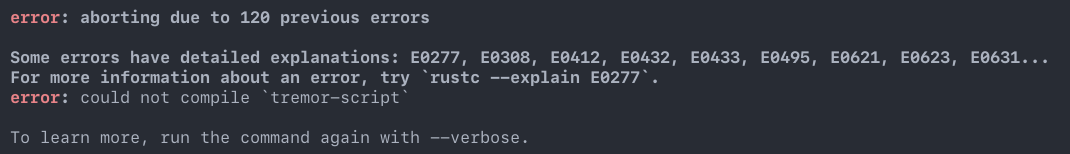
\includegraphics[width=\textwidth]{./Imagenes/errors.png}
    \caption{Al intentar evitar los tipos externos se produjeron más de 120
    errores de compilación.}%
    \label{fig:errors}
\end{figure}

\subsubsection{Encapsular el tipo externo}

Otra opción es crear un \emph{wrapper} para \code{halfbrown}, de la misma forma
que lo hace ya \abistable con otras librerías más conocidas. Este
encapsulamiento hace posible su uso desde el ABI de C de forma segura. Sin
embargo, estos ejemplos ya existentes son complejos~\cite{complexwrapper} y
difíciles de mantener, ya que tendrán que actualizarme con cada nueva versión de
\code{halfbrown}.

\subsubsection{Reimplementar el tipo con el ABI de C desde cero}

Similar a la solución anterior, pero con incluso más costoso, dado que también
requeriría reimplementar la funcionalidad. Puede parecer indeseable, pero es la
mejor forma de asegurar un rendimiento máximo. Los tipos externos mencionados
son parte de optimizaciones; encapsularlos podría tener un impacto en su
rendimiento y hacerlos inútiles.

Si esta parte del proyecto es lo suficientemente importante y existen los
recursos, debería considerarse. De hecho, el mismo tipo \rust{Value} en Tremor
surgió por esta razón: ya existía \rust{simd_json::Value} de otra librería, pero
carecía de la suficiente flexibilidad y el equipo implementó uno personalizado.

\subsubsection{Simplificar el tipo para la interfaz}

Esta última opción resultó ser la más sencilla de implementar: crear una copia
de \rust{Value} cuyo único uso es para comunicarse entre runtime y plugins,
ilustrado en la Figura~\ref{fig:simplify}.

\begin{figure}
    \centering
    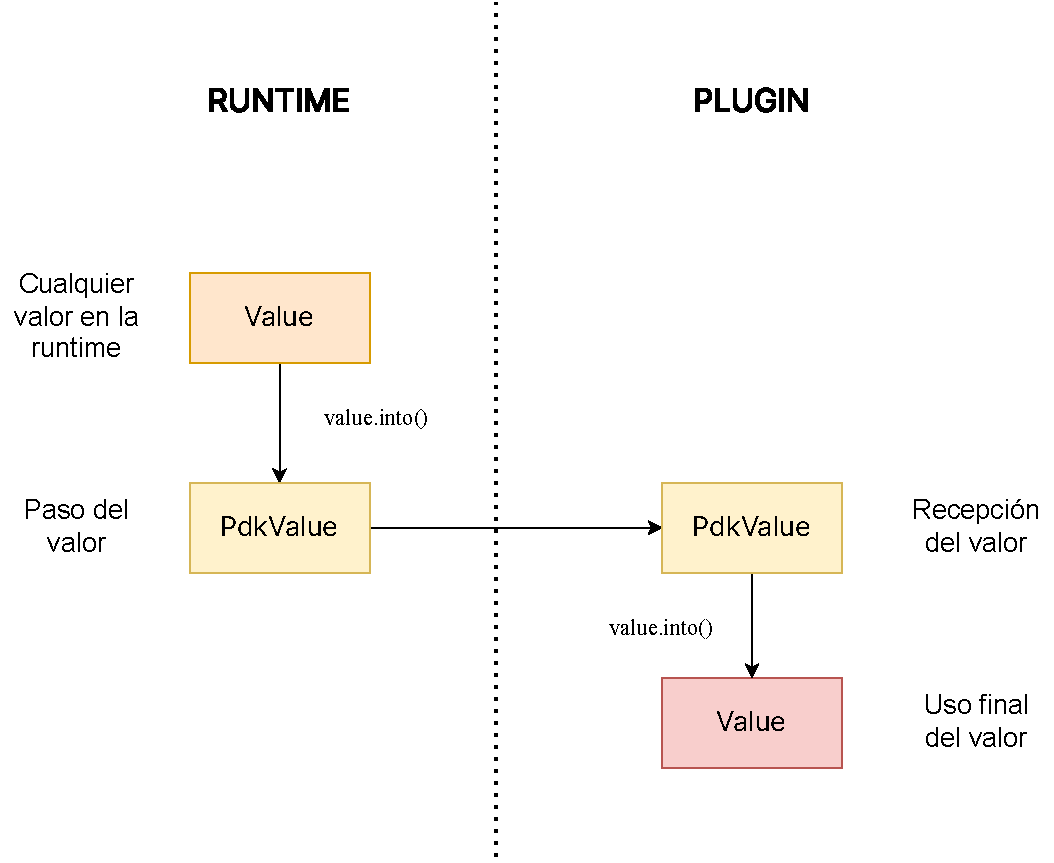
\includegraphics[width=10cm]{./Imagenes/simplify.pdf}
    \caption{Comunicación entre runtime y plugins en el PDK.}%
    \label{fig:simplify}
\end{figure}

Ya que es un tipo nuevo, no se romperá nada del código ya existente, y
únicamente hará falta cambiarlo donde se use la interfaz. Su implementación es
sencilla (notar el cambio de nombre a \rust{PdkValue}):

\begin{minted}{rust}
pub enum PdkValue {
    /// Valores estáticos (enteros, booleanos, etc)
    Static(StaticNode),
    /// Tipo para cadenas de caracteres
    String(String),
    /// Tipo para listas
    Array(Vec<Value>),
    /// Tipo para objetos (mapas clave-valor)
    Object(Box<HashMap<String, PdkValue>>),
    /// Tipo para datos binarios
    Bytes(Vec<u8>),
}
\end{minted}

No es necesario escribir métodos adicionales para el nuevo \rust{PdkValue}, solo
sus conversiones desde y hasta el tipo original, \rust{Value}. Esto sería
equivalente a, en vez de pasar un \rust{Vec<T>} al PDK, reemplzarlo con un
\rust{*const u8} para los datos y un \rust{u32} para la longitud. Simplemente
consiste en simplificar los tipos en la interfaz, y convertirlos de vuelta para
usar la funcionalidad completa.

El problema principal es que la conversión entre tipos es ahora $O(n)$ en vez de
$O(1)$, dado que es necesario iterar los datos en los objetos y vectores para la
conversión. Su uso sería el siguiente:

TODO: mejor si omito el siguiente snippet de código?

\begin{minted}{rust}
// Esta función es exportada por el plugin. Funcionará porque
// `PdkValue` está declarado con el ABI de C.
pub extern "C" fn plugin_funfuncue: PdkValue) {
    let value = Value::from(value);
    value.do_func()
}

// Esto se puede implementar en la runtime para facilitar su uso,
// convirtiendo al tipo original.
fn runtime_wrapper(value: Value) {
    plugin_func(value.into());
}
\end{minted}

Es la alternativa más sencilla, pero implica un coste de rendimiento; dos
conversiones implican iterar los datos dos veces. Tras mediciones posteriores,
se verificó que convertir los datos era un 5-10\% de la ejecución del programa.
Es menos de lo esperado, pero sigue sin ser suficiente para Tremor.

También tiene un coste de usabilidad; en comparación con tener un único
\rust{Value}, es necesario convertir los tipos y posiblemente crear encapsularlo
con una función de más alto nivel (\rust{runtime_wrapper}). Es una tarea
relativamente trivial, por lo que se podría automatizar con macros procedurales
en Rust, pero esto debería dejarse para el final del proyecto.

En conclusión, esta alternativa es la más fácil de implementar en el corto
plazo y por tanto la que mejor sigue \work. Una vez esté terminado, se puede
analizar el rendimiento y optar por una alternativa más eficiente, como
reescribir los tipos para el caso de uso específico de Tremor.

\subsection{Problemas con varianza y subtipado}

Otro problema inesperado tuvo que ver con la \emph{varianza} y \emph{subtipado}.
Son dos conceptos de teoría de sistemas de tipos, especialmente conocidos por
desarrolladores de lenguajes orientados a objetos como Java o C\#. En el caso de
Rust solo se da en las \lifetimes, así que no es tan popular. Lo que lo hace más
complicado de tratar es que es completamente implícito: mejora la usabilidad del
lenguaje cuando \emph{funciona}; en caso contrario, resulta en errores
intricados y difíciles de identificar.

Este tema no se cubre en \textcite{rustbook}, sino en \textcite[Subtyping and
Variance]{nomicon} y \textcite[Subtyping and Variance]{rustref}. También es
recomendable consultar el artículo \textcite{lcnr_covandcontra} o a
\textcite{video_covandcontra} para un formato en vídeo.

Deriva también de los problemas encontrados con el tipo \rust{Value}. La
historia completa se incluye en el issue \textcite{abi_covandcontra}. Al cambiar
los tipos de la librería estándar a los de \abistable, se producían errores de
\lifetimes \emph{inexplicables} (ver Figura~\ref{fig:errors}). Estuve bloqueado
con dicho problema durante mucho tiempo, así que tras comentárselo a mis
mentores, Heinz me ayudó a reproducir el problema de forma mínima. Por alguna
razón que todavía desconocíamos, dos tipos supuestamente equivalentes diferían a
la hora de compilar:

\begin{minted}{rust}
use abi_stable::std_types::RCow;
use std::borrow::Cow;

fn cmp_cow<'a, 'b>(left: &Cow<'a, ()>, right: &Cow<'b, ()>) -> bool {
    left == right
}

// Este caso falla en compilación, pero es aparentemente igual
fn cmp_rcow<'a, 'b>(left: &RCow<'a, ()>, right: &RCow<'b, ()>) -> bool {
    left == right
}
\end{minted}

\begin{minted}{text}
$ cargo build
error[E0623]: lifetime mismatch
  --> src/lib.rs:10:10
   |
9  | fn cmp_rcow<'a, 'b>(
   |        left: &RCow<'a, ()>, right: &RCow<'b, ()>) -> bool {
   |              ------------          ------------
   |              |
   |              these two types are declared with
   |              different lifetimes...
10 |     left == right
   |          ^^ ...but data from `left` flows into `right` here

For more information about this error, try `rustc --explain E0623`.
error: could not compile `repro` due to previous error
\end{minted}

Este tipo de error suele darse en caso de que la \lifetime de un valor no viva
lo suficiente. Por ejemplo, el ejemplo de \code{rustc --explain E0623} es el
siguiente. Se tienen dos \lifetimes \emph{sin relación entre sí}, \rust{'short}
y \rust{'long}. La estructura \rust{Foo} que se pasa como parámetro tiene la
\lifetime \rust{'short}, pero dentro de la función se le intenta asignar una
\lifetime \rust{'long}, que es imposible porque el compilador no sabe cuál tiene
un tiempo de vida mayor. Asignarle una \lifetime que viva más de lo que debe
significaría que se podría seguir usando \rust{Foo} después de que \rust{'short}
acabe, es decir, después de que \rust{Foo} haya sido destruido. Finalmente, esto
causaría inconsistencias en memoria porque nuestra variable de tipo \rust{Foo}
ya no existe, pero se está intentando acceder a ella.

\begin{minted}{rust}
struct Foo<'a> {
    x: &'a isize,
}

fn bar<'short, 'long>(c: Foo<'short>, l: &'long isize) {
    // Equivalente a asignarle otra lifetime a c
    let c: Foo<'long> = c; // error!
}
\end{minted}

Solucionarlo es tan simple como indicar que \rust{'short} tiene al menos el
mismo tiempo de vida que \rust{'long}. Es decir, que no se podría dar el caso de
que \rust{Foo} es usado después de destruirse:

\begin{minted}{rust}
// Notar que ahora `'short` se declara tal que `'short: 'long`
fn bar<'short: 'long, 'long>(c: Foo<'short>, l: &'long isize) {
    let c: Foo<'long> = c; // ok!
}
\end{minted}

Por tanto, uno pensaría que tiene que ver con el operador \rust{==}, que se
delega al \trait \rust{PartialEq}, así que dediqué tiempo intentando encontrar
la diferencia entre su implementación en \rust{Cow<'a, T>} y la de
\rust{RCow<'a, T>}. La mención anterior a estos errores como
\emph{inexplicables} se debe a que en este caso únicamente existe una \lifetime
\rust{'a}, así que no se podría arreglar indicando que \rust{'short: 'long}. No
obstante, existía alguna pequeña diferencia sin relación a este problema entre
las implementaciones, y al usar \emph{exactamente lo mismo} que en \rust{Cow<'a,
T>}, compilaba correctamente.

% TODO: credit properly
Tras cambiar \rust{left == right} por \rust{left.cmp(right)} en la reproducción
inicial, se repetía el problema, incluso con aparentemente la misma
implementación de \rust{Ord} (el \trait con el método \rust{cmp}). No fue hasta
que expliqué mi problema en un servidor de Discord con más desarrolladores de
Rust que descubrí que el verdadero problema era un término llamado la
\emph{varianza} de \rust{RCow<'a, T>}.

Todo acabó reduciéndose a la única diferencia en la implementación del \trait
\rust{Ord}. \rust{RCow<'a, T>} implementa un \trait llamado
\rust{BorrowOwned<'a>} y \rust{Cow<'a, T>} implementa otro llamado
\rust{ToOwned}. Ambos \traits son iguales, excepto que en \rust{BorrowOwned<'a>}
se incluye funcionalidad adicional para \abistable. El problema no tiene que ver
con esta diferencia en funcionalidad, sino que \rust{BorrowOwned<'a>} es
genérico respecto a la \lifetime \rust{'a}, lo cual no es el caso de
\rust{ToOwned}.

Al implementar \rust{Ord}, se tenía que indicar que \rust{T: ToOwned} o \rust{T:
BorrowOwned<'a>}. El problema era que al relacionar la \lifetime \rust{'a} de
esta forma, estaba rompiendo una regla que hacía a \rust{RCow}
\emph{invariante}, en vez de \emph{covariante}.

TODO: es esta sección demasiado técnica? Debería continuar? Me falta explicar
qué es invarianza y covarianza. La verdad que esto sí que me llevó mucho tiempo
en su momento, así que me gustaría incluirlo de alguna forma.

\section{Estado final del proyecto}

Como se ha explicado, la complejidad del proyecto resultó ser mucho mayor que lo
esperado por problemas con el ABI. Por tanto, resultó imposible desarrollar en
el tiempo disponible un sistema de plugins tan completo y eficiente como se
especificaba.

La última versión del sistema de plugins es funcional y, mediante contribuciones
de código abierto, ha hecho posible su futura inclusión en una versión de
Tremor. Muchas de las librerías usadas no disponían de la funcionalidad
necesaria para este proyecto, así como \code{async_ffi}, \code{abi_stable},
\code{halfbrown} o \code{simd-json}.

El problema principal tiene que ver con el rendimiento. Dada la naturaleza de
Tremor, es un requerimiento imprescindible para poderlo incluir en una futura
versión. Tras unas mediciones iniciales, se calculó que su inclusión reducía el
rendimiento del programa un 30\%, así que los siguientes pasos consistieron en
reducir dicha cifra.

TODO: incluir todas las figuras de benchmarks con las explicaciones

% vim: spelllang=es

\chapter{Implementación}

\section{Metodología}

Antes de nada, es importante aprender un poco sobre cómo realizar cambios en el
código de Tremor eficientemente. Este proyecto modificará gran cantidad de
líneas y cuanto más rápido sea el desarrollo, menos problemas habrán. Esto se
puede cubrir de forma específica al lenguaje Rust, con trucos o consejos que
puedan facilitar el desarrollo, o de forma más general, con la estrategia de
trabajo a seguir. En esta sección se cubrirá lo último, dado que es menos un
detalle de implementación.

La metodología fue insipirada por mis mentores, que lo denominaron el ``Just
Make it Work'', o \work. Se basa en que, inicialmente, con lo que más problemas
tenía era el perderme en los detalles. Pero ciertamente, primero de todo lo
importante es que ``funcione''. Siempre y cuando el sistema de plugins se pueda
compilar y ejecutar, lo siguiente es secundario:

\begin{itemize}
    \item Código ``feo'' (no idiomático, repetitivo o desordenado).

    \item Código de bajo rendimiento.

    \item Documentación pobre.

    \item No tener tests prematuros.

    \item No aplicar sugerencias recomendadas por \emph{linters} (en el caso de
        Rust, \emph{Clippy}).

\end{itemize}

El propio desarrollo invitaba a aprovechar las ventajas de un lenguaje
fuertemente tipado como Rust, evitando realizar testing posiblemente prematuro.
Esto consistía en realizar cambios y posteriormente trabajar en que los aceptara
el compilador, repetidamente. Únicamente se procedió al testing exhaustivo una
vez la interfaz final del sistema de plugins compilaba, pasadas las fases
tempranas o incluso medias.

Adicionalmente, las optimizaciones prematuras son la fuente de todos los
problemas. No es algo que sea importante aún. Solo una vez terminada la primera
iteración se puede dedicar más tiempo a medir el rendimiento para saber cuáles
optimizaciones merecen la pena. Notar que sí es importante escoger un
\emph{método o tecnología} que sea apropiado en términos de rendimiento; fue por
ello por lo que se descartó WebAssembly o IPC en el capítulo anterior. Pero
definitivamente el desarrollador debería rendirse en, por ejemplo, evitar una
conversión entre dos tipos innecesaria que posiblemente no afecte al rendimiento
al fin y al cabo.

Lo que quería dejar claro el equipo de Tremor es que todos los tests, limpiezas
u optimizaciones que intentes realizar en este momento acabará muy probablemente
siendo en vano. Se llegará a un punto en el que no se pueda continuar y que
requiera repensar y reescribir gran parte del trabajo. Cuando todo compile y
aparentemente funcione correctamente, se puede dedicar esfuerzo a trabajar en
estos temas secundarios. Si algo no importante está llevando demasiado tiempo,
se debería marcar como TODO o FIXME y dejarlo para otro momento.

Notar que no hay problema con ``gastar'' el tiempo con métodos que acaban siendo
incorrectos, porque realmente no se está ``gastando'' nada; son un paso
necesario para llegar a la solución final. Pero es doloroso tener que eliminar
código al que le has dedicado tiempo, así que al menos debería intentarse
minimizar el impacto que esto tenga.

\section{Versionado en \abistable}

Dado que \abistable va a ser la librería principal en la que se basará el
sistema de plugins, es importante entender cómo funciona al completo. Además de
conocer los detalles de implementación, es importante conocer cómo \abistable
soluciona los problemas a tener en cuenta para implementar un sistema de
plugins. La librería especifica lo siguiente respecto a su sistema de
compatibilidad de tipos~\cite{abistable_safety}:

\begin{itemize}
    \item El ABI de \abistable se comprueba siempre. Cada versión \code{0.y.0} y
        \code{x.0.0} de \abistable define su propio ABI, que es incompatible
        con versiones anteriores.

    \item Los tipos se comprueban recursivamente cuando se carga una librería
        dinámica, antes de llamar ninguna función.

\end{itemize}

Todo esto se basa en el \trait (equivalente en este caso a una clase abstracta
de Java) \rust{StableAbi}, indicador de que un tipo es seguro para cargado
dinámico. Contiene información como su disposición en memoria y puede ser
implementado automáticamente con un macro. Al cargar un plugin con \abistable,
se comprobará que sus tipos sean compatibles con aquellos de la runtime.

Sin este mecanismo, sería posible cargar un plugin con una interfaz diferente a
la runtime, resultando en violaciones de acceso a memoria. Pongamos un caso en
el que una estructura en la interfaz de la runtime tuviese un campo adicional.
El plugin exportará esa estructura sin el campo nuevo, puesto que usa una
interfaz anticuada. Cuando la runtime intente acceder a la estructura del
plugin, se leerá un campo que no existe y que por tanto es parte de memoria no
definida.

\section{Conversión de la interfaz a C}

Es importante mantener la interfaz de plugins lo más simple posible. Los
detalles de comunicación deberían dejarse a la runtime, de forma que los plugins
se limiten a exportar una lista de funciones síncronas. De esta forma, se podrá
evitar en lo posible pasar tipos complejos (programación asíncrona, canales de
comunicación, etc) entre la runtime y los plugins, que implicaría una carga de
trabajo mucho más alta.

Una vez esta interfaz de bajo nivel se defina, se puede crear un \emph{wrapper}
de más alto nivel en la runtime que se encargue de la comunicación y de mejorar
su usabilidad dentro de Tremor. Esto mismo lo hacen otras \crates como
\cratelink{rdkafka}, que implementa una capa de abstracción asíncrona sobre su
interfaz de C en \cratelink{rdkafka-sys}.

El primer paso consiste en declarar la interfaz del PDK de forma que use el ABI
de C, en vez del de Rust. Esto se puede hacer con el atributo \rust{#[repr(C)]}
(en lugar del \rust{#[repr(Rust)]} implícito). Para usar \abistable también
tendrá que implementarse el \trait \rust{StableAbi}.

La dificultad reside en que todos los tipos dentro de la interfaz \emph{también}
tendrán que haber sido declarados con tanto \rust{#[repr(C)]} como
\rust{StableAbi}, recursivamente. Esto puede convertirse en un problema si
alguno de los tipos a convertir es externo y no se tiene acceso directo. Tendrá
que abrirse un pull request para añadir soporte, o crear un \emph{wrapper} que
envuelva la funcionalidad de forma opaca a su distribución en memoria. Se
incluye la explicación completa respecto a Tremor en el Anexo~\ref{annex:abi},
con más detalles sobre la implementación.

\section{Cargado de plugins}

Afortunadamente, \abistable ya se encarga de la mayoría del trabajo en este
aspecto. Lo único que hace falta implementar es una manera en la que
\emph{encontrar} los plugins en el sistema. Para ello, se introduce una nueva
variable de entorno \code{TREMOR_PLUGIN_PATH} que liste todos los directorios
que pueden contener plugins. De forma similar a \code{PATH}, los directorios se
separan con dos puntos.

Una vez se tiene la lista de directorios, se comprobarán también sus
subdirectorios, recursivamente. Es importante añadir un límite de profundidad
aquí para evitar que el programa se quede atascado, por ejemplo si el usuario
incluyese el directorio raíz (\code{/}) accidentalmente. Tampoco deberían
seguirse enlaces simbólicos por simplicidad.

Todos aquellos archivos encontrados cuya extensión sea la de una librería
dinámica tendrán que añadirse a la lista de posibles plugins. Esta extensión
varía según el sistema operativo: en Linux es \code{.so}, en Windows es
\code{.dll}, y en MacOS es \code{.dylib}.

Finalmente, si al intentar cargar uno de los plugins encontrados la operación
falla, se mostrará una advertencia y se continuará hasta probar con todas las
ocurrencias. Un método más robusto para evitar cargar ficheros que no sean
plugins de Tremor sería usar una extensión personalizada, o algun tipo de
convención para el nombre. Sin embargo, al personalizarse manualmente los
directorios, se asume que la gran mayoría de las librerías dinámicas serán
plugins.

\section{Gestión de pánicos}\label{sec:panics}

Los pánicos en Rust se usan para expresar errores de los que un programa no se
puede recuperar. Por ejemplo, acceder a un índice inexistente en una lista, o
quedarse sin memoria. Su funcionamiento es similar a una excepción de C++ o
Java: se propagarán hasta llegar a la función principal y parar la ejecución del
programa.

Actualmente, lanzar pánicos a través de la interfaz C es comportamiento no
definido~\cite[FFI and Panics]{nomicon}. Aunque el programa aborte en la mayoría
de los casos, no existe ninguna garantía de que vaya a suceder así; podría
continuar en un estado inválido, con cualquier tipo de consecuencia.

La solución más directa es usar la función \rust{std::panic::catch_unwind}, que,
para casos excepcionales como este, puede parar la propagación de pánicos cuando
sea llamada. Se podría usar en todas las funciones exportadas por el plugin
internamente, y en caso de producirse un pánico se terminaría el programa
manualmente, en lugar de dejar que se propague a la runtime, que sería
indefinido.

También es posible configurar el programa por completo para que aborte cuando se
produzca un pánico, en vez de propagarlo. De esta forma, no se llegaría a
invocar comportamiento no definido y se mantendría un rendimiento máximo ---
capturar pánicos tiene un coste. Sin embargo, implica varias desventajas
importantes: al abortar, no se tendrá acceso a la información de \emph{debug}
que dan los pánicos, tampoco se limpiará el estado del programa, y desde la
runtime es imposible saber si el plugin ha configurado los pánicos para que
aborten. Esto último será posible en el futuro, una vez
\textcite{pluggablepanic} llegue a una versión estable.

Esto es algo que \abistable ha tenido en cuenta desde el principio. Antes de que
un pánico se vaya a propagar de plugin a runtime, la librería abortará el
programa por completo. Esta parte se realiza transparentemente; no hace falta
que el desarrollador se preocupe en ningún momento por ello.

La solución de \abistable no es perfecta, ya que tiene un pequeño coste de
rendimiento e imposibilita el recuperarse de errores en los plugins. En una
futura versión de Tremor, podría ser posible reiniciar plugins en caso de que
dejen de funcionar para mejorar la resiliencia a fallos.

El equipo de Rust conoce esta limitación y está trabajando en mejorar la
situación. En una futura versión, planea definir cuándo se puede propagar un
pánico de forma más precisa~\cite{cunwind}.

\section{Programación asíncrona}

El objetivo inicial era simplificar la interfaz lo suficiente como para que no
sea necesario tratar aspectos como programación asíncrona en el PDK. Esto
terminó siendo inevitable, dado que la asincronía es uno de los pilares de
Tremor.

Para poder usar programación asíncrona con el ABI de C se puede recurrir a la
\crate \cratelink{async_ffi}, cuyo único problema era no tener soporte para
\abistable en concreto. Al no implementar el \trait \rust{StableAbi}, no se
podía usar en la interfaz del PDK, por lo que tuve que abrir un pull request
para hacerlo yo mismo~\cite{asyncfficontrib}. El uso de esta librería resulta en
código más verboso, pero esto se podría mejorar en el futuro con
macros~\cite{asyncffimacro}.

\section{Seguridad en hilos}

\abistable utiliza la \crate \cratelink{libloading} internamente, cuya gestión
de errores no es segura en hilos en algunas plataformas, como \code{dlerror} en
FreeBSD~\cite{thsafe_libloading}\cite{thsafe_openbsd}. Sí que lo es en
Linux~\cite{thsafe_linux}, macOS~\cite{thsafe_macos} y Windows~\cite{thsafe_ms},
así que en el caso de Tremor no es un problema.

Será importante tenerlo en cuenta en el futuro; al añadir soporte para un nuevo
sistema operativo habrá que asegurarse de que su gestión de errores sea segura
en hilos. En caso contrario, deberá actualizarse \code{libloading} para
sincronizar el acceso con un mútex interno, como lo hace la \crate
\cratelink{dlopen}~\cite{thsafe_dlopen}. Notar que \code{dlopen} es también
mejorable, dado que usa el mútex \emph{siempre}, incluso en sistemas operativos
donde la gestión de errores sí es segura en hilos~\cite{thsafe_dlopen_issue}.

\section{Complejidad de las conversiones}\label{abiperf}

Un punto vital a tener en cuenta es el coste de realizar conversiones entre
tipos de la librería estándar y tipos de \abistable. Esto se dará en numerosas
ocasiones, dado que usar \abistable cuando no es necesario es subóptimo para
tanto el rendimiento como la usabilidad. Y si, por ejemplo, convertir un
\rust{Vec<T>} a un \rust{RVec<T>} tuviese complejidad $O(n)$, probablemente
\abistable tendría que ser descartado como la solución escogida.

Afortunadamente, tras analizar la implementación de tipos como \rust{RVec<T>},
\rust{RSlice<T>}, \rust{RStr} o \rust{RString}, estas conversiones únicamente
consisten en transferir un puntero con los datos, sin necesidad de copiar nada.
Es decir, las conversiones que realizaremos serán $O(1)$.

\section{Problemas con varianza y subtipado}

Una complicación a la que se dedicó una cantidad considerable de tiempo tiene
que ver con el concepto de \emph{varianza} y \emph{subtipado}. En resumen, si un
tipo es \emph{covariante}, el modelo de memoria de Rust será mucho más flexible
al usarlo. Todo este mecanismo es implícito, es decir, en ningún momento el
desarrollador especifica manualmente la varianza del tipo; el compilador de Rust
lo infiere automáticamente.

Sin embargo, un tipo puede dejar de ser covariante si incumple una serie de
reglas preestablecidas. En ese caso, la flexibilidad adicional se pierde y se
producen errores casi imposibles de entender si uno no es familiar con el
término \emph{varianza}. Los tipos definidos en \abistable, a diferencia de
aquellos en la librería estándar, no eran covariantes, lo cual fue especialmente
complicado de descubrir y requirió reescribir algunas partes suyas por completo.

Afortunadamente, una futura versión de Rust hará el debugging de estos errores
mucho más intuitivo~\cite{smarterchecker}. Es un tema que requiere conocimientos
más avanzados de Rust, por lo que se incluye en el Anexo~\ref{annex:covariance}
al completo para más información.

\section{Optimizaciones}

Una vez implementada la primera versión del sistema de plugins, se realizan
optimizaciones iterativamente hasta alcanzar un rendimiento lo suficientemente
bueno. Esto incluye una limpieza general del código, la restauración de
optimizaciones que se eliminaron temporalmente (ver Anexo~\ref{annex:abi}) o la
simplificación de la interfaz del PDK.

% vim: spelllang=es

\chapter{Conclusiones y trabajo futuro}

\section{Concusiones}

La complejidad del proyecto ha resultado ser mucho mayor de lo esperado,
principalmente por el malentendido sobre la estabilidad del ABI de Rust. Por
tanto, ha resultado imposible desarrollar en el tiempo disponible un sistema de
plugins tan completo y eficiente como se especificaba inicialmente.

El problema principal tiene que ver con el rendimiento. Dada la naturaleza de
Tremor, es un requerimiento imprescindible para poderlo incluir en producción.
Tras las pruebas realizadas en el Anexo~\ref{annex:benchmarks}, se ha calculado
que el sistema de plugins reduce el rendimiento un 30\%.

No obstante, la última versión del sistema de plugins es perfectamente funcional
y, mediante su investigación, el diseño de su arquitectura y contribuciones de
código abierto, se ha hecho posible su inclusión en una futura versión de
Tremor.

Parte de esta ralentización en el desarrollo se debe también a Rust. Al ser un
lenguaje tan inmaduro es frecuente encontrar documentación pobre o librerías
incompletas. Muchas de las \crates usadas no disponían inicialmente de la
funcionalidad necesaria para un sistema de plugins, como \code{async_ffi},
\code{abi_stable}, \code{halfbrown} o \code{simd-json}. Se han resuelto
problemas importantes en el entorno, extendiendo el soporte para el ABI de C,
resolviendo tipos con varianzas inflexibles y elaborando conversiones de tipos
no triviales, todo ello manteniendo la máxima seguridad y eficiencia posible.
Con esfuerzos como estos, el desarrollo de proyectos similares en el futuro
resultará mucho más accesible.

\section{Futuro}

Se ha documentado tanto el proceso seguido como lo que queda pendiente, de forma
que el equipo de Tremor pueda continuar trabajando en el sistema de plugins para
su futuro lanzamiento. Sin embargo, aun después de esto el PDK nunca parará de
evolucionar: su uso se extenderá en la base de código y se perfeccionarán otras
características con el tiempo. Algunas ideas son las siguientes:

\begin{itemize}
    \item \textbf{Mejoras de rendimiento}: el enfoque principal para el primer
        lanzamiento del PDK. Esto incluye la realización de \emph{benchmarks}
        más variados y realistas, y el soporte de \abistable en más librerías.

    \item \textbf{Soporte de otros componentes de Tremor}: el PDK únicamente se
        implementa para los conectores, pero también podría funcionar con
        códecs, preprocesadores, postprocesadores, operadores, funciones,
        extractores, etc.

    \item \textbf{Refinamiento de la experiencia de usuario}: creación de
        proyectos modelo como base para plugins nuevos, ejemplos de uso, macros,
        documentación exhaustiva y de más alto nivel, frameworks de testing,
        etc.

    \item \textbf{Carga de plugins a petición del usuario}: además de poder
        cargar los plugins al inicio del programa, sería especialmente útil
        solicitar su carga durante la ejecución. Se podría elaborar un nuevo
        método de configuración iterativo, en el que se cargan y configuran los
        plugins uno a uno, y finalmente se exporta la composición final.

    \item \textbf{Paquetes de plugins}: en ciertos casos, sería más conveniente
        exportar un plugin que implemente más de un componente. Por ejemplo,
        podrían juntarse los conectores de TCP y UDP en único plugin, dado que
        probablemente compartan partes de su código y dependencias.

    \item \textbf{Gestión de versiones alternativas}: la implementación de
        \abistable para comprobar las versiones es rudimentaria y poco
        eficiente; se limita a comprobarlos todos recursivamente. Otra opción
        más simple sería únicamente comprobar una cadena con el versionado
        global para la interfaz, por ejemplo.

    \item \textbf{Mayor seguridad}: el cargado dinámico no ofrece ningún tipo de
        aislamiento sobre los plugins y no es adecuado si estos no son de
        confianza. Si en una futura versión de WebAssembly su rendimiento
        mejorase considerablemente, se podría volver a considerar su uso.

    \item \textbf{Registro centralizado de plugins}: en el futuro a largo plazo,
        se podría desarrollar una funcionalidad similar a los repositorios de
        Maven o Cargo. Allí se podrían guardar todos los plugins de la comunidad
        para gestionarlos automáticamente.

    \item \textbf{Eliminación de plugins en tiempo de ejecución}: es
        especialmente complejo de implementar, dado que \abistable
        explícitamente no lo soporta. Sin embargo, esto mejoraría
        considerablemente la resiliencia a errores, siendo posible reiniciar
        plugins completamente.

\end{itemize}

\section{Valoración personal}

Pese a las situaciones de frustración frente a todos los errores y bloqueos que
he encontrado en el camino, ha sido una experiencia extraordinaria. Matthias
bromeó una vez con que ``El infierno de debugging es importante para el
desarrollo de personaje'', y creo que tiene toda la razón. Enfrentarme a errores
que no sabía ni cómo abordar me ha enseñado mucho sobre Rust, y lo que es más
importante, sobre desarrollo de software en general.

Estoy muy satisfecho con haber conseguido lo que he conseguido, y aún más por
haberlo poder hecho junto al increíble equipo que es el de Tremor. Trabajar con
ellos me ha ayudado a descubrir qué quiero hacer tras la graduación, y con qué
tipo de empresa y personas quiero trabajar. Me mantendré en contacto con ellos
para seguir el progreso del sistema de plugins.

\endgroup

% BIBLIOGRAFÍA Y REFERENCIAS
\printbibliography%
\nocite{*} % Include all the entries in the bibliography, even if not mentioned

% ANEXOS

% Vuelta a configurar los párrafos para que no afecte al índice
\setlength{\parskip}{\baselineskip}%
\setlength{\parindent}{0pt}%

\newpage
\appendix
\clearpage
\addappheadtotoc%
\appendixpage%
\chapter{Guía de Rust}\label{annex:rust}

Es posible que en este anexo se omitan algunos conceptos o que algunas
explicaciones no sean completamente precisas por razones de simplicidad.
\namecite{rustbook} es el libro oficial para aprender Rust por completo, pero es
una lectura larga y posiblemente demasiado exhaustiva. Para mayor brevedad, se
recomienda leer \namecite{rustprofessionals}, \namecite{rustgentleintro} o
\namecite{rust30min}.

La comunidad dispone de otros libros que explican aspectos más avanzados del
lenguaje en específico, como \unsafe o la programación asíncrona. En esos casos,
se recomienda leer \namecite{nomicon} y \namecite{rustasyncbook},
respectivamente.

\section{Primeros pasos}

Comenzando por el clásico ``Hola Mundo'', se incluyen algunos ejemplos de cómo
es la sintaxis de Rust más básica. Los binarios o librerías en Rust reciben el
nombre de \crate. Nuestra \crate se podría ejecutar fácilmente con \emph{Cargo},
el administrador de dependencias oficial, o específicamente con el comando
\code{cargo run}.

\begin{minted}{rust}
fn main() {
    println!("Hello World!");
}
\end{minted}

\code{main} es nuestra función principal, que invoca al macro \code{println!}
para escribir por pantalla. Notar que la invocación de macros, a diferencia de
funciones, requiere un \rust{!} al final.

\section{Conceptos principales}

Los bloques básicos (\rust{if}, \rust{else}, \rust{while}, \rust{for}) son muy
similares a en otros lenguajes. También existe \rust{match}, que permite extraer
patrones de variables.

\begin{minted}{rust}
fn factorial(i: u64) -> u64 {
    match i {
        // Primer caso: i = 0
        0 => 1,
        // El resto de casos, asignado a una variable `n`
        n => n * factorial(n-1)
    }
}
\end{minted}

Uso de variables y métodos:

\begin{minted}{rust}
fn main() {
    // Declaración de una variable, cuyo tipo se infiere
    // automáticamente.
    let my_number = 1234;
    // Declaración de una variable con un tipo especificado
    // manualmente. Notar que se puede usar el mismo nombre, y la
    // variable anterior será destruida.
    let my_number: i32 = 4321;
    // Invocación de la función estática (constructor) `new` dentro
    // del tipo `String`. El uso de `mut` indica que la instancia del
    // tipo se puede modificar. Funciona de forma inversa a C++, que
    // por defecto es mutable y `const` indica que *no* se puede
    // modificar.
    let mut my_str = String::new();
    // Invocación del método `push` de `my_str`, que añade un
    // carácter al final de la cadena.
    my_str.push('a');
}
\end{minted}

Otros componentes principales de Rust son:

\begin{itemize}
    \item Estructuras de datos:

\begin{minted}{rust}
struct MessageA {
    // Campo público con una cadena de caracteres
    pub text: String,
    // Campo privado con un entero
    user_id: i32,
}
\end{minted}

\begin{minted}{rust}
// Sin nombres de campos; se pueden acceder con `data.0`
// y `data.1`, respectivamente.
struct MessageB(pub String, i32);
\end{minted}

    \item Enumeraciones, que también permiten contener datos:

\begin{minted}{rust}
enum MessageC {
    Join,
    Text(String, i32),
    Leave(i32),
}
\end{minted}

    \item \emph{Traits}, similares a las interfaces de Java en el sentido de que
        son una serie de requerimientos y que un tipo puede implementar
        múltiples \traits, pero también permiten implementaciones por defecto:

\begin{minted}{rust}
trait Sender {
    // Los métodos requieren especificar `self` explícitamente,
    // que es lo mismo que `this` en Java o C++. En este caso,
    // `&send` tomará una referencia al tipo que implemente
    // `Sender`. También podría ser una referencia mutable con
    // `&mut self`, o el mismo tipo con `self`.
    fn send(&self, msg: String);

    // Implementación por defecto.
    fn send_twice(&self, msg: String) {
        self.send(msg);
        self.send(msg.clone());
    }
}
\end{minted}

        Y para implementar un trait para un tipo:

\begin{minted}{rust}
impl Sender for MessageC {
    fn send(&self, msg: String) {
        match self {
            Join => println!("Joined"),
            Text(txt, id) => println!("{} sent: {}", id, txt),
            // Las variables `_` son ignoradas
            Leave(_) => println!("Left"),
        }
    }

    // `send_twice` se implementará automáticamente.
}
\end{minted}

    Notar que, sin embargo, Rust no es un lenguaje orientado a objetos. Un
    \trait puede heredar de otro \trait, pero un \struct no puede heredar de
    otro \struct.

\end{itemize}

\section{Genéricos y librería estándar}

De forma similar a C++, Rust posee tipos genéricos. Esto permite la
implementación de una librería estándar flexible, con varias estructuras de
datos importantes a conocer:

% NOTE: esto creo que lo puedo evitar si no incluyo cómo se usa async_ffi, que
% me parece demasiado complejo para el documento.
% \begin{minted}{rust}
% // Función genérica, donde `ToString` es un trait
% fn print<T: ToString>(t: T) {}

% // Otra manera de especificar genéricos con diferencias
% // menores que no se explicarán en esta introducción.
% fn print(t: impl ToString) {}
% \end{minted}

\begin{itemize}
    \item Tipos primitivos:
        \begin{itemize}
            \item Carácteres con \rust{char}.

            \item Punto flotante con \rust{f32} y \rust{f64}.

            \item Booleanos con \rust{bool}.

            \item Enteros: \rust{u8}, \rust{i8}, \rust{u16}, \rust{i16},
                \rust{u32}, \rust{i32}, \rust{u64}, \rust{i64}, e incluso
                \rust{i128} y \rust{u128} en las arquitecturas que lo soportan.

            \item Vectores de tamaño fijo: por ejemplo \rust{[1, 2, 3, 4, 5]}.

            \item N-tuplas como \rust{(1, true, 9.2)}.

            \item El tipo ``unidad'', \rust{()}, equivalente a \code{void} en C
                o C++.

            \item Punteros básicos con \rust{*const T} o \rust{*mut T}.

        \end{itemize}

    \item \rust{Vec<T>} representa un vector contiguo y redimensionable.

    \item \rust{HashMap<K, V>} es una tabla hash, genérica respecto a su clave
        \rust{K} y su valor \rust{V}. No se encuentra en el preludio, por lo que
        requeriría la siguiente declaración, similar a un \code{import} de Java:

\begin{minted}{rust}
use std::collections::HashMap;
\end{minted}

    \item \rust{Box<T>}, usado para localizar un tipo \rust{T} no nulo en
        memoria. Además de un \rust{*const T}, incluye el tamaño que ocupa
        \rust{T} y tiene una interfaz limitada para que su uso sea siempre
        seguro.

    \item \rust{str} es una cadena UTF-8 de solo lectura, típicamente usada con
        una referencia \rust{&str}. Va acompañada por su longitud, por lo que no
        hace falta terminarla con \code{\0}, a diferencia de C. \rust{String} es
        su versión modificable asignada en memoria.

\end{itemize}

\section{Gestión de errores}

En Rust, los errores se indican con el tipo \rust{Result<T, E>}. Este se trata
de una enumeración cuyo valor puede ser \rust{Ok(T)}, con el resultado obtenido
satisfactoriamente, o \rust{Err(E)}, con el tipo de error que ha sucedido. Dado
que el resultado está contenido dentro suyo, es imposible olvidar comprobar si
se ha producido algún error. Se puede usar \rust{match} para comprobar el
resultado, o una serie de funciones disponibles para hacer el proceso más
ergonómico:

\begin{minted}{rust}
match load_file(input) {
    Ok(data) => /* ... */,
    Err(e) => eprintln!("Error: {e}"),
}
\end{minted}

En caso de que se produjera un error del que el programa no se puediera
recuperar, como quedarse sin memoria o un fallo inesperado en la implementación,
se usa la funcionalidad de \emph{pánicos}. Un pánico se propaga de forma similar
a una excepción de C++ o Java, y terminará la ejecución por completo. Se puede
invocar con el macro \rust{panic!} o utilidades similares.

\section{Macros}

Rust cuenta con dos tipos de macros: \emph{declarativos} y \emph{procedurales}.
Ambos permiten generar código a tiempo de compilación, pero se diferencian
principalmente en la flexibilidad que ofrecen, a coste de un coste de desarrollo
menor o mayor, respectivamente.

Los macros declarativos se crean con una sintaxis especializada, similar a un
\rust{match} con patrones de tokens (identificadores, tipos, etc) como entrada,
y los tokens nuevos como salida. Son similares a los macros de C o C++, pero más
potentes e higiénicos (i.e., su expansión no captura identificadores
accidentalmente).

Los macros procedurales se describen como extensiones del lenguaje.
Esencialmente, ejecutan código en la compilación que consume y produce sintaxis
de Rust; consisten en directamente transformar el Árbol de Sintaxis Abstracta
(AST)~\cite[Procedural Macros]{rustref}. Consecuentemente, su complejidad es
mucho mayor, pero expanden las posibilidades de los macros enormemente.

\begin{minted}{rust}
some_macro!(1, 2, 3); // Puede ser tanto declarativo como procedural
\end{minted}

\begin{minted}{rust}
// Sintaxis típica de invocación de un macro
some_macro! {
    fn some_function() { /* ... */ }
}

// También permitido en el caso de los procedurales
#[some_macro]
fn some_function() { /* ... */ }
\end{minted}

Finalmente, los macros procedurales se pueden declarar de forma que
\emph{deriven} (implementen automáticamente) un \trait. Esto evita escribir
código repetitivo de forma muy sencilla:

\begin{minted}{rust}
// Con un macro `derive` para el trait `Debug`, que sirve para
// mostrar variables por pantalla.
#[derive(Debug)]
struct X(i32);

// Sin ellos sería lo siguiente. Como es trivial se puede
// simplificar en un macro procedural de tipo `derive`.
impl fmt::Debug for X {
    fn fmt(&self, f: &mut fmt::Formatter) -> fmt::Result {
        write!(f, "{:?}", self.0)
    }
}
\end{minted}

\section{Lifetimes}

La seguridad que provee Rust en memoria se basa en un modelo a tiempo de
compilación con \lifetimes. Una \lifetime es 

TODO: esto depende de cómo se acaba incluyendo la sección de ``problemas con
varianza y subtipado''.

\section{Unsafe}

Para poder mantener control completo a bajo nivel, es posible ignorar sus
garantías de seguridad con el sub-lenguaje llamado \emph{unsafe Rust}. El
análisis estático de Rust es conservativo; en algunas ocasiones es posible que
rechace algunos programas correctos. El desarrollador puede indicar que es
consciente de la situación y puede apagar este análisis para corregirlo por sí
mismo, arriesgándose a cometer un error en su código.

Se puede acceder a \emph{unsafe Rust} conteniendo el código dentro de un bloque
\rust{unsafe { /* ... */ }} o una función \rust{unsafe fn name() { /* ... */ }}.
Funciona igual que rust, pero incluye varias nuevas habilidades, entre otras:

\begin{itemize}
    \item Leer un puntero bruto en memoria

    \item Acceder o modificar una variable estática mutable

    \item Llamar a una función \unsafe

\end{itemize}

\section{Programación asíncrona}

Como muchos lenguajes modernos, Rust da soporte a la programación asíncrona, un
modelo de programación concurrente. Sin entrar en excesivo detalle, esta permite
tener una gran cantidad de \emph{tareas} concurrentes ejecutándose sobre unos
pocos hilos del Sistema Operativo. Su caso de uso principal es programas cuyo
rendimiento está limitado por operaciones de entrada y salida, como servidores o
bases de datos~\cite{rustasyncbook}.

\begin{minted}{rust}
// Con `async` se indica que la función es asíncrona.
async fn get_two_sites_async() {
    // Creación de dos "futuros" que, al completarse, descargarán
    // asíncronamente las páginas web. Similar a la creación de
    // un nuevo hilo.
    let future_one = download_async("https://www.foo.com");
    let future_two = download_async("https://www.bar.com");

    // Ejecutar las dos tareas. Similar a esperar la terminación de
    // los hilos.
    join!(future_one, future_two);

    // Con `.await` se puede esperar a la terminación de un futuro
    // individual.
    let future_three = download_async("https://www.bar.com").await;
}
\end{minted}

\chapter{Funcionamiento interno de Tremor}\label{annex:tremor}

\section{Arquitectura}

Antes de comenzar a modificar el código existente en Tremor, era importante
conocer cómo funciona para evitar perder el tiempo. Tremor se basa en el modelo
actor. Citando Wikipedia:

TODO: puedo citar Wikipedia?

% ORIGINAL:
% ``[The actor model treats the] actor as the universal primitive of concurrent
% computation. In response to a message it receives, an actor can: make local
% decisions, create more actors, send more messages, and determine how to
% respond to the next message received. Actors may modify their own private
% state, but can only affect each other indirectly through messaging (removing
% the need for lock-based synchronization).''

``[El modelo actor trata al] actor como el componente universal de computación
concurrente. En respuesta a un mensaje que recibe, un actor puede: tomar
decisiones locales, crear más actores, enviar más mensajes y determinar cómo
responder al siguiente mensaje recibido. Los actores pueden modificar su propio
estado privado, pero solo pueden afectarse entre sí indirectamente a través de
mensajería (eliminando la necesidad de sincronización con
\emph{locks}).''~\cite{wikiactor}

No usa un lenguaje (e.g., Erlang) o framework (e.g., \cratelink{bastion}, quizá
en el futuro) que siga estrictamente este modelo, pero re-implementa los mismos
patrones frecuentemente de forma manual. Tremor se basa en \emph{programación
asíncrona}, es decir, que en vez de hilos trabaja con \emph{tareas}, un concepto
de nivel más alto y especializado para entrada/salida. De la documentación de
\cratelink{async-std}, la runtime asíncrona que usa Tremor:

% ORIGINAL:
% ``An executing asynchronous Rust program consists of a collection of native OS
% threads, on top of which multiple stackless coroutines are multiplexed. We
% refer to these as “tasks”. Tasks can be named, and provide some built-in
% support for synchronization.''

``La ejecución de un programa asíncrono en Rust consiste en una recopilación de
hilos nativos del Sistema Operativo, sobre los cuales múltiples corutinas no
apilables (\emph{stackless}) son multiplexadas. Nos referimos a ellas como
``tareas''. Las tareas pueden tener nombre e incluir soporte para
sincronización.''~\cite{asyncstd_task}

Podríamos resumir su arquitectura con la frase ``Tremor se basa en actores
corriendo en tareas diferentes, que se comunican asíncronamente con canales''.

\section{Detalles de implementación}

El actor principal se llama \rust{World}. Contiene el estado del programa, como
los artefactos disponibles (\emph{repositorios}) y los que se están ejecutando
(\emph{registros}) y se usa para inicializar y controlar el programa.

Los \emph{managers} o \emph{gestores} son simplemente actores en el sistema que
envuelven una funcionalidad. Ayudan a desacoplar la comunicación y la
implementación de la funcionalidad interna. De esta forma, se puede eliminar
código repetitivo al inicializar los componentes, así como la creación de
canales de comunicación o el lanzamiento del componente en una tarea nueva.
Generalmente, hay un gestor por cada tipo de artefacto para facilitar su
inicialización y también uno por cada instancia que se esté ejecutando, para
controlar su comunicación.

Notar que la inicialización de los conectores ocurre en dos pasos. Primero se
\emph{registran}, es decir, se indica su disponibilidad para cargarlo
(añadiéndolo al repositorio). Posteriormente, no se ejecutará hasta conectarse
con otro artefacto con \rust{launch_binding}, lo cual lo movería del repositorio
al registro, junto al resto de artefactos ejecutándose.

\begin{figure}[h]
    \centering
    \begin{minted}{rust}
pub trait Connector {
    /// Crea la parte "source" del conector, si es aplicable.
    async fn create_source(
        &mut self,
        _source_context: SourceContext,
        _builder: source::SourceManagerBuilder,
    ) -> Result<Option<source::SourceAddr>> {
        Ok(None)
    }

    /// Crea la parte "sink" del conector, si es aplicable.
    async fn create_sink(
        &mut self,
        _sink_context: SinkContext,
        _builder: sink::SinkManagerBuilder,
    ) -> Result<Option<sink::SinkAddr>> {
        Ok(None)
    }

    /// Intenta conectarse con el mundo exterior. Por ejemplo, inicia la
    /// conexión con una base de datos.
    async fn connect(
        &mut self,
        _c: &ConnectorContext,
        _attempt: &Attempt
    ) -> Result<bool> {
        Ok(true)
    }

    /// Llamado una vez cuando el conector inicia.
    async fn on_start(&mut self, _c: &ConnectorContext) -> Result<()> {
        Ok(())
    }
    /// Llamado cuando el conector pausa.
    async fn on_pause(&mut self, _c: &ConnectorContext) -> Result<()> {
        Ok(())
    }
    /// Llamado cuando el conector continúa.
    async fn on_resume(&mut self, _c: &ConnectorContext) -> Result<()> {
        Ok(())
    }
    /// Llamado ante un evento de "drain", que se asegura de que no
    /// lleguen más eventos a este conector.
    async fn on_drain(&mut self, _c: &ConnectorContext) -> Result<()> {
        Ok(())
    }
    /// Llamado cuando el conector para.
    async fn on_stop(&mut self, _c: &ConnectorContext) -> Result<()> {
        Ok(())
    }
}
    \end{minted}
    \caption{Simplificación del \trait \rust{Connector}}%
    \label{fig:tremor_connector_trait}
\end{figure}

\subsection{Registro}

La Figura~\ref{fig:tremor_registering} detalla todos los pasos seguidos en el
código. Primero han de inicializarse los gestores, y después registrar los
artefactos. Actualmente, esta parte se realiza de forma estática con
\rust{register_builtin_types}, pero después de implementar el PDK, debería ser
dinámicamente. Tremor buscaría automáticamente plugins en sus directorios
configurados e intentaría registrar todos los que encuentre. En una futura
versión, el usuario podría solicitar manualmente el cargado de un plugin nuevo
mientras se está ejecutando Tremor.

\begin{figure}
    \centering
    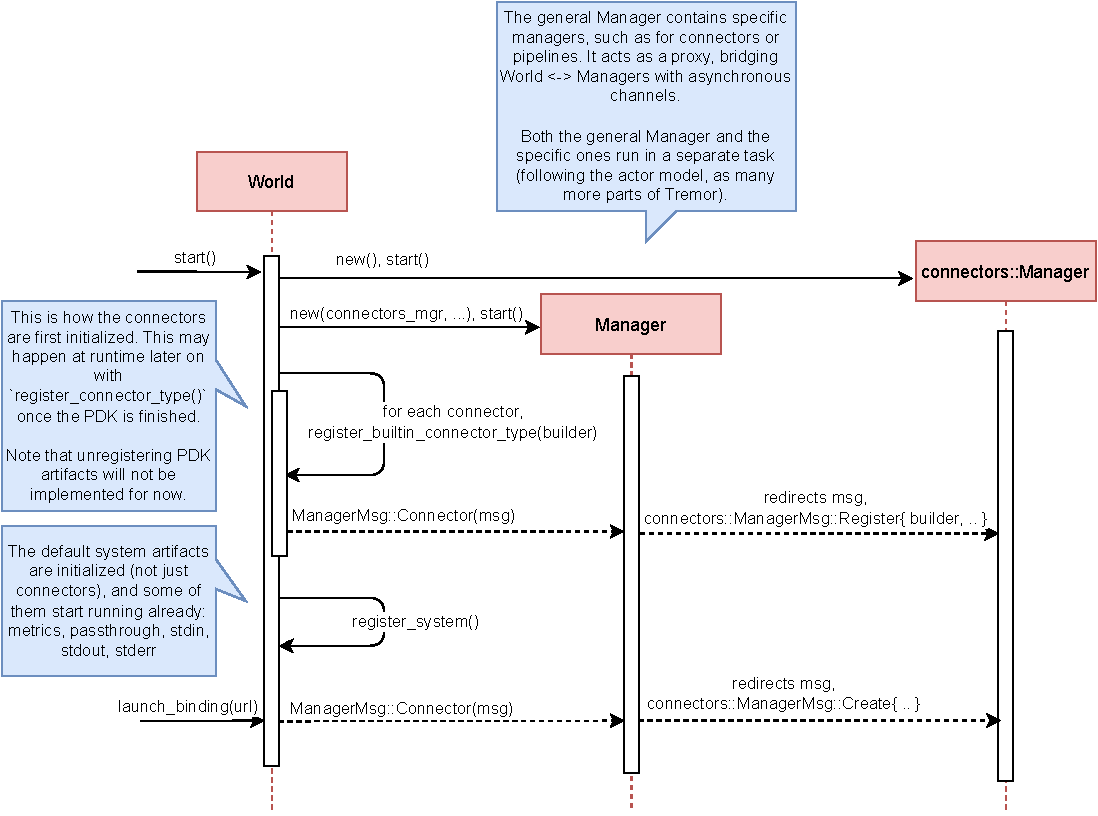
\includegraphics[width=\textwidth]{./Imagenes/registering.pdf}
    \caption{Registro de un conector en el programa}%
    \label{fig:tremor_registering}
\end{figure}

\subsection{Inicialización}

Ya que es un proceso en múltiples pasos (en la implementación es más complicado
que registro + creación), la primera parte provee las herramientas para
inicializar el conector (el \emph{builder}). Cuando el conector necesite
comenzar a ejecutarse porque se haya añadido a una \pipeline, el \builder ayuda
a construir y configurarlo de forma genérica. Finalmente, se añade a una tarea
propia para que se pueda comunicar con otras partes de Tremor. El gestor
\rust{connectors::Manager} contiene todos los conectores ejecutándose en Tremor,
como se muestra en la Figura~\ref{fig:tremor_initializing}.

\begin{figure}
    \centering
    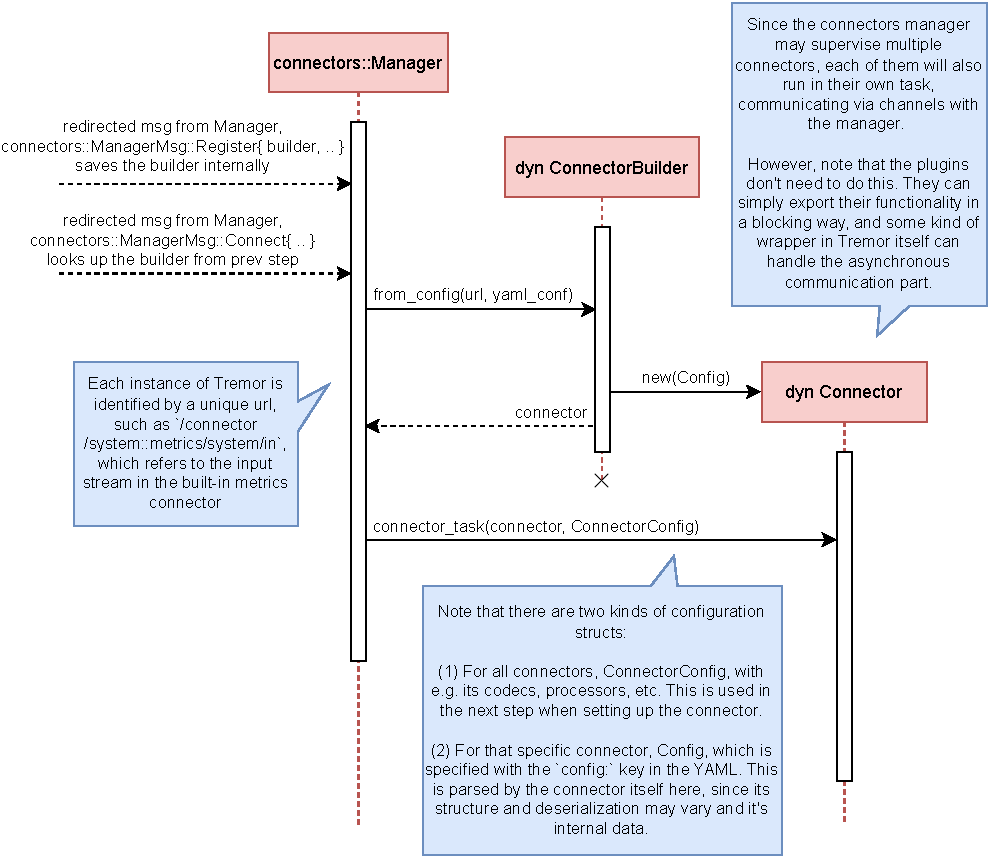
\includegraphics[width=\textwidth]{./Imagenes/initializing.pdf}
    \caption{Inicialización de un conector en el programa}%
    \label{fig:tremor_initializing}
\end{figure}

\subsection{Configuración}

Una vez haya un conector corriendo, la Figura \ref{fig:tremor_setting_up}
visualiza cómo se divide en una parte \sink y otra \source. Estas son
opcionales, pero no exclusivas, así que se puede tener cualquiera de las dos o
ambas. De forma similar, un \builder se usa para inicializar las partes y a
continuación inicia una nueva tarea para ellos.

\begin{figure}
    \centering
    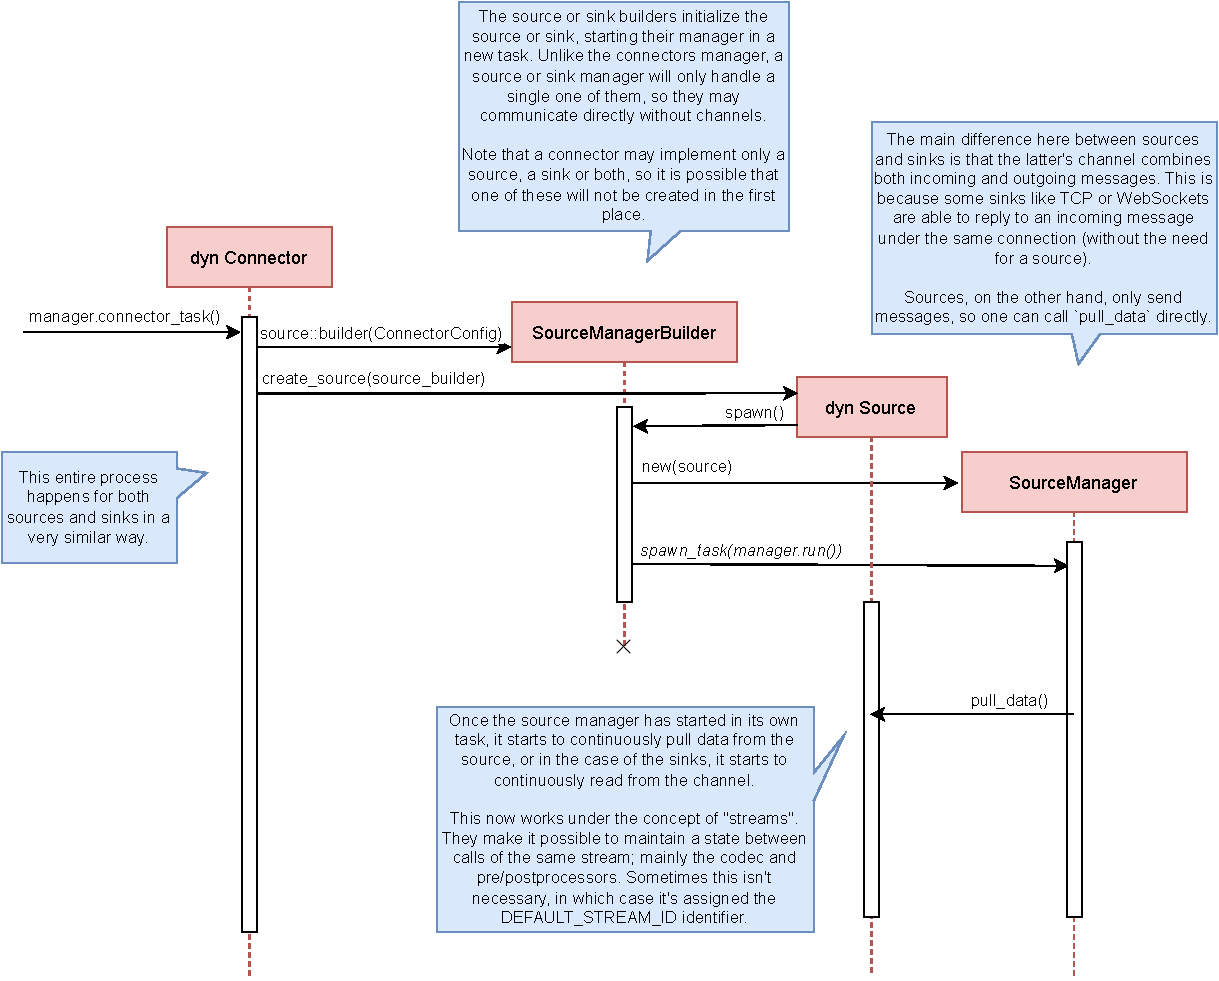
\includegraphics[width=\textwidth]{./Imagenes/setting-up.pdf}
    \caption{Configuración de un conector en el programa}%
    \label{fig:tremor_setting_up}
\end{figure}

También se crea un gestor por cada instancia de \sink o \source, que se
encargará de la comunicación con otros actores. De esta forma, sus interfaces
pueden mantenerse lo más simple posible. Esos gestores recibirán peticiones de
conexión de la \pipeline y posteriormente leerán o enviarán eventos en ella.

La diferencia principal entre \sources y \sinks a nivel de implementación es que
este último también puede responder a mensajes usando la misma conexión. Esto es
útil para notificar que el paquete ha llegado (\rust{Ack}) o que algo ha fallado
(\rust{Fail} para un evento específico, \rust{CircuitBreaker} para dejar de
recibir datos por completo).

Los códecs y preprocesadores se involucran aquí tanto para los \sources como
para los \sinks. En la parte de \source, los datos son transformados a través de
una cadena de preprocesadores y posteriormente se aplica un códec. Para los
\sinks, se sigue el proceso inverso: los datos se codifican primero a bytes con
el códec, y posteriormente una serie de postprocesadores se aplican a los datos
binarios.

\subsection{Notas adicionales}

Algunos conectores se basan en \emph{flujos}. Son equivalentes a los flujos de
TCP, que ayudan a agrupar mensajes para evitar mezclarlos. Se inician y
finalizan mediante mensajes, y el gestor se guarda el estado del flujo en un
campo llamado \rust{states} (ya que, por ejemplo, algunos preprocesadores puedan
querer guardar un estado). Si un conector no necesita flujos, como
\rust{metronome} (que únicamente envía eventos periódicamente), puede
especificar su identificador de flujo como \rust{DEFAULT_STREAM_ID} siempre.

Tras implementar la interfaz de los conectores para el sistema de plugins,
los primeros conectores a desarrollar deberían ser:

\begin{itemize}
    \item \emph{Blackhole}, usado para medir el rendimiento. Realiza mediciones
        de tiempos de final a final para cada evento pasando por la \pipeline, y
        al final guarda un histograma HDR (\emph{High Dynamic Range}).

    \item \emph{Blaster}, usado para repetir una serie de eventos de un archivo,
        que es especialmente útil para pruebas de rendimiento.

\end{itemize}

Ambos son relativamente simples y serán de gran ayuda para medir el efecto de
los cambios sobre el rendimiento. De todos modos, el equipo de Tremor insistía
que lo más importante primero es que funcione, y después me podría preocupar
sobre eficiencia.

\chapter{Conversión del ABI de Rust al ABI de C}\label{annex:abi}

Para ilustrar mejor el problema de conversión de ABIs, se introduce la
estructura más complicada al respecto, \rust{Value}. Esta estructura sirve para
representar datos pseudo-JSON y es definido a continuación de forma
simplificada:

\begin{minted}{rust}
pub enum Value {
    /// Valores estáticos (enteros, booleanos, etc)
    Static(StaticNode),
    /// Tipo para cadenas de caracteres
    String(String),
    /// Tipo para listas
    Array(Vec<Value>),
    /// Tipo para objetos (mapas clave-valor)
    Object(Box<HashMap<String, Value>>),
    /// Tipo para datos binarios
    Bytes(Vec<u8>),
}
\end{minted}

Para poder usar \rust{Value} en la interfaz del sistema de plugins, se puede
convertir a:

\begin{minted}{rust}
#[repr(C)] // La representación en memoria de Value seguirá el ABI de C
#[derive(StableAbi)] // Solo necesario cuando se usa abi_stable
pub enum Value {
    Static(StaticNode),
    /// Ahora usa `RString`, la altenativa a `String` de abi_stable
    String(RString),
    /// De forma similar, usa `RVec` en vez de `Vec`
    Array(RVec<Value>),
    /// Cambio de `Box`, `HashMap` y `String` por sus alternativas
    Object(RBox<RHashMap<RString, Value>>),
    /// Otro cambio de `Vec`
    Bytes(RVec<u8>),
}
\end{minted}

El primer problema surge en la variante \rust{Static}. Su tipo contenido
internamente, \rust{StaticNode}, es externo y usa \rust{#[repr(Rust)]}. Se
declara en el \crate \cratelink{value_trait}, que lo declara tal que:

\begin{minted}{rust}
pub enum StaticNode {
    I64(i64),
    U64(u64),
    F64(f64),
    Bool(bool),
    Null,
}
\end{minted}

Esto se podría arreglar siguiendo el mismo procedimiento recursivamente, hasta
que todo sea \rust{#[repr(C)]}. Pero como se trata de una librería externa,
tendrá que abrirse un nuevo pull request y esperar que al autor le parezcan bien
los cambios~\cite{openstaticnode}. Será importante también que la estructura use
\rust{#[repr(C)]} únicamente cuando opcionalmente se configure a tiempo de
compilación como necesario. De esta forma, el resto de usuarios podrán seguir
aprovechándose de las ventajas de rendimiento que ofrece \rust{#[repr(Rust)]}.

\section{Consecuencias del sistema de plugins}

Por desgracia, este cambio no termina ahí; cambiar las variantes de \rust{Value}
implica que el código que lo usaba se romperá de numerosas formas:

\begin{minted}{rust}
// No funcionará porque Value::Array contiene un RVec ahora
let value = Value::Array(Vec::new());
\end{minted}

Este caso es el más sencillo: simplemente hace falta cambiar \rust{Vec} por
\rust{RVec}. La intención de los tipos de \abistable es que sean un reemplazo
directo de los de la librería estándar, i.e., su interfaz será la misma:

\begin{minted}{rust}
let value = Value::Array(RVec::new());
\end{minted}

TODO: 'return' es devolver o retornar?

Es un poco más complicado cuando los tipos anteriores se exponían en métodos,
porque requiere tomar una decisión entre expandir el límite de FFI del
\emph{funcionamiento interno} de \rust{Value} a los \emph{usuarios} de
\rust{Value}. Por ejemplo, la variante \rust{Value::Object} contiene un
\rust{RHashMap} ahora, pero el método \rust{Value::as_object} solía devolver una
referencia a \rust{HashMap}. Se producirá un error nuevo ahí y tendrá que
tomarse la decisión de devolver \rust{RHashMap} o añadir una conversión interna
a \rust{HashMap}:

\begin{minted}{rust}
impl Value {
    // Código original
    fn as_object(&self) -> Option<&HashMap<String, Value>> {
        match self {
            // Problema: `m` ahora es una `RHashMap`, pero la función
            // devuelve un `HashMap`.
            //
            // Solución 1: cambiar el tipo devuelto a `RHashMap`
            // Solución 2: convertir `m` a un `HashMap` con `m.into()`
            Self::Object(m) => Some(m),
            _ => None,
        }
    }
}
\end{minted}

\begin{itemize}
    \item Si se cambia el tipo devuelto a \rust{RHashMap}, casi todas las veces
        que se llamaba a \rust{as_object} ahora dejarán de compilar porque se
        esperan un \rust{HashMap}.

        Esto puede ser complicado porque, para evitar realizar conversiones, el
        sistema de plugins \emph{infectaría} la base de código por completo.
        Tendría que propagarse el uso de \rust{RHashMap} por todo el programa,
        incluso cuando el PDK no es importante. Por ejemplo, \rust{Value}
        también se usaba en la implementación del lenguaje de Tremor, Troy.
        Tener que usar un \rust{RHashMap} en esa situación sería confuso y
        acabarían modificándose gran cantidad de ficheros sin relación al
        sistema de plugins.

    \item Si se realiza una conversión interna a \rust{HashMap} en
        \rust{as_object}, evitaremos todos esos errores, con un pequeño coste de
        rendimiento. Es la opción más fácil, pero si \rust{Value::as_object} se
        usara frecuentemente, e.g., en el bucle principal, sí que podría causar
        una degradación considerable.
\end{itemize}

Como indica la sección~\ref{abiperf}, las conversiones entre la librería
estándar y \abistable son $O(1)$. Esto es dónde la metodología \work es
relevante: simplemente dejaremos el límite del FFI en su mínimo y añadiremos
conversiones cuanto antes sea posible. Al terminar, si se detectan problemas de
rendimiento en un caso en concreto, se puede reconsiderar.

\section{Problemas con tipos externos}\label{sec:abi_ext}

En algunos casos, los tipos de \abistable no habían sido actualizados para
incluir métodos nuevos de la librería estándar, por lo que era necesario un pull
request para añadirlo\footnote{El anexo \ref{annex:contributions} lista todas
las contribuciones de código abierto realizadas para este proyecto}. Pero por lo
general, convertir los tipos \emph{de la librería a estándar a \abistable} es
una tarea trivial, simplemente un tanto tedioso.

Los problemas surgen cuando es necesario convertir \emph{tipos externos a
\abistable}. La declaración anterior de \rust{Value} era una simplificación;
realmente, Tremor usa la implementación de \cratelink{halfbrown} de
\rust{HashMap<K, V>}. Esto se debe a que es más eficiente para su caso de uso, y
que posee algunas funcionalidades adicionales necesarias. El mismo caso se da
para otro tipo \rust{Cow}, cuya alternativa en la \crate \cratelink{beef} ocupa
menos espacio en memoria y ofrece un mejor rendimiento en Tremor.

Ninguno de estos dos tipos tienen soporte dentro de \abistable, y aunque estos
tipos estén basados en otros de la librería estándar, la conversión no es
directa. Se pueden tomar cuatro posibles alternativas:

\subsection{Evitar el tipo externo}

Basándose en \work, una solución perfectamente válida es eliminar las
optimizaciones temporalmente y dejar un \code{TODO} para que se pueda revisar
posteriormente. Es posible que el sistema de plugins tenga excesiva complejidad,
y limitarse a usar tipos de la librería estándar podría ser suficiente.

En el caso específico de \rust{Value}, eliminar las optimizaciones problemáticas
parece la manera más fácil de arreglar el problema. Y lo sería, si no fuera
porque eliminar código también puede ser complicado, como muestra la
Figura~\ref{fig:errors}, especialmente cuando la funcionalidad extra del tipo
externo no está disponible.

\begin{figure}
    \centering
    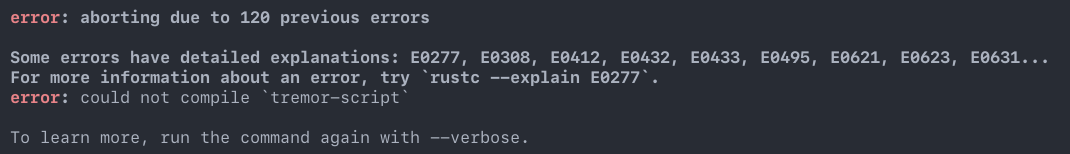
\includegraphics[width=\textwidth]{./Imagenes/errors.png}
    \caption{Al intentar evitar los tipos externos se produjeron más de 120
    errores de compilación.}%
    \label{fig:errors}
\end{figure}

\subsection{Encapsular el tipo externo}

Otra opción es crear un \emph{wrapper} para \code{halfbrown}, de la misma forma
que lo hace ya \abistable con otras librerías más conocidas. Este
encapsulamiento hace posible su uso desde el ABI de C de forma segura. Sin
embargo, estos ejemplos ya existentes son complejos~\cite{complexwrapper} y
difíciles de mantener, ya que tendrán que actualizarme con cada nueva versión de
\code{halfbrown}.


\begin{figure}
    \centering
    \begin{minted}{rust}
// Así funciona la programación asíncrona en Rust; la primera
// función es prácticamente equivalente a la segunda.
async fn example() -> String {
    read_file().await
}
fn example() -> impl Future<Output = String> {
    async {
        read_file().await
    }
}

// No pueden haber genéricos en FFI, por lo que ahora `Future`
// es un tipo concreto `FfiFuture` en vez de un trait. La
// conversión de `Future` a `FfiFuture` se puede realizar con
// `into_ffi`.
fn example() -> FfiFuture<String> {
    async move {
        read_file().await
    }
    .into_ffi()
}
// `FfiFuture<T>` implementa `Future<Output = T>`, por lo que
// su uso es el mismo.
async fn user() {
    example().await
}
    \end{minted}
    \caption{Interfaz modificada para la programación asíncrona en el sistema de
    plugins con la \crate \code{async_ffi}.}%
    \label{fig:async_ffi}
\end{figure}

\subsection{Reimplementar el tipo con el ABI de C desde cero}

Similar a la solución anterior, pero con incluso más costoso, dado que también
requeriría reimplementar la funcionalidad. Puede parecer indeseable, pero es la
mejor forma de asegurar un rendimiento máximo. Los tipos externos mencionados
son parte de optimizaciones; encapsularlos podría tener un impacto en su
rendimiento y hacerlos inútiles.

Si esta parte del proyecto es lo suficientemente importante y existen los
recursos, debería considerarse. De hecho, el mismo tipo \rust{Value} en Tremor
surgió por esta razón: ya existía \rust{simd_json::Value} de otra librería, pero
carecía de la suficiente flexibilidad y el equipo implementó uno personalizado.

\subsection{Simplificar el tipo para la interfaz}

Esta última opción resultó ser la más sencilla de implementar: crear una copia
de \rust{Value} cuyo único uso es para comunicarse entre runtime y plugins,
ilustrado en la Figura~\ref{fig:simplify}.

\begin{figure}
    \centering
    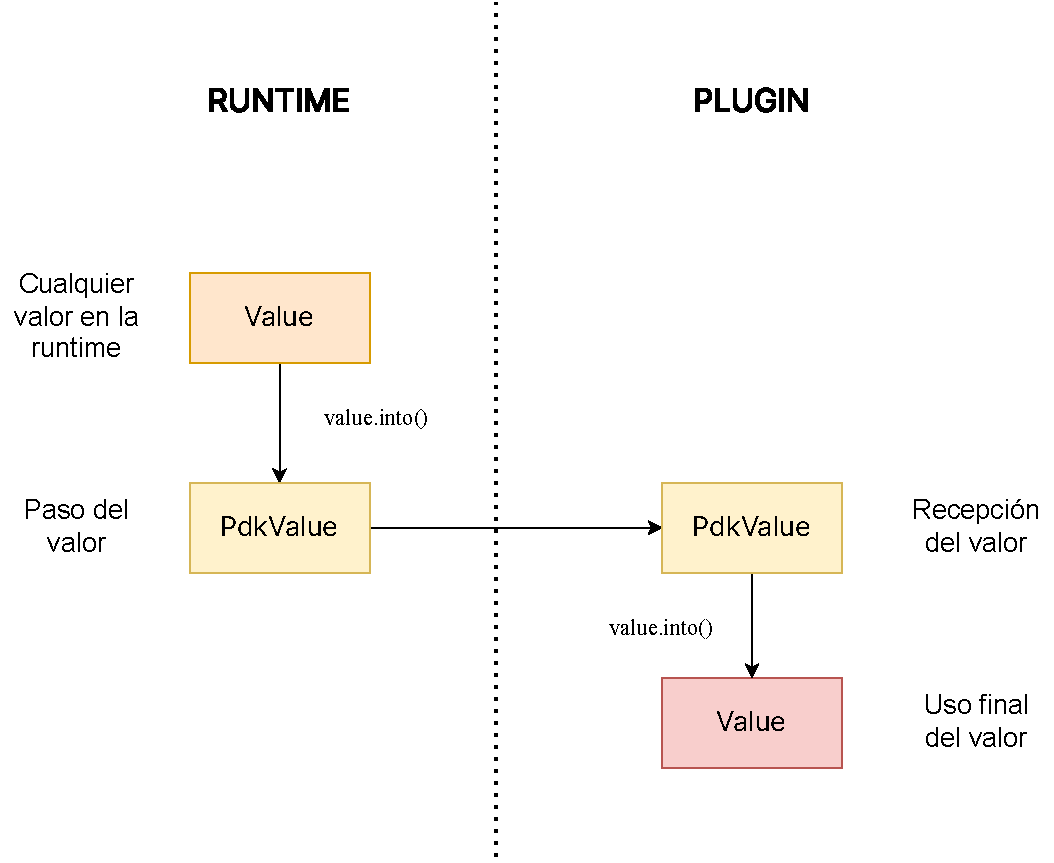
\includegraphics[width=10cm]{./Imagenes/simplify.pdf}
    \caption{Comunicación entre runtime y plugins en el PDK.}%
    \label{fig:simplify}
\end{figure}

Ya que es un tipo nuevo, no se romperá nada del código ya existente, y
únicamente hará falta cambiarlo donde se use la interfaz. Su implementación es
sencilla (notar el cambio de nombre a \rust{PdkValue}):

\begin{minted}{rust}
pub enum PdkValue {
    /// Valores estáticos (enteros, booleanos, etc)
    Static(StaticNode),
    /// Tipo para cadenas de caracteres
    String(String),
    /// Tipo para listas
    Array(Vec<Value>),
    /// Tipo para objetos (mapas clave-valor)
    Object(Box<HashMap<String, PdkValue>>),
    /// Tipo para datos binarios
    Bytes(Vec<u8>),
}
\end{minted}

No es necesario escribir métodos adicionales para el nuevo \rust{PdkValue}, solo
sus conversiones desde y hasta el tipo original, \rust{Value}. Esto sería
equivalente a, en vez de pasar un \rust{Vec<T>} al PDK, reemplzarlo con un
\rust{*const u8} para los datos y un \rust{u32} para la longitud. Simplemente
consiste en simplificar los tipos en la interfaz, y convertirlos de vuelta para
usar la funcionalidad completa.

El problema principal es que la conversión entre tipos es ahora $O(n)$ en vez de
$O(1)$, dado que es necesario iterar los datos en los objetos y vectores para la
conversión. Su uso sería el siguiente:

\begin{minted}{rust}
// Esta función es exportada por el plugin. Funcionará porque
// `PdkValue` está declarado con el ABI de C.
pub extern "C" fn plugin_funfuncue: PdkValue) {
    let value = Value::from(value);
    value.do_func()
}

// Esto se puede implementar en la runtime para facilitar su uso,
// convirtiendo al tipo original.
fn runtime_wrapper(value: Value) {
    plugin_func(value.into());
}
\end{minted}

Es la alternativa más sencilla, pero implica un coste de rendimiento; dos
conversiones implican iterar los datos dos veces. Tras mediciones posteriores,
se verificó que convertir los datos era un 5-10\% de la ejecución del programa.
Es menos de lo esperado, pero sigue sin ser suficiente para Tremor.

También tiene un coste de usabilidad; en comparación con tener un único
\rust{Value}, es necesario convertir los tipos y posiblemente crear encapsularlo
con una función de más alto nivel (\rust{runtime_wrapper}). Es una tarea
relativamente trivial, por lo que se podría automatizar con macros procedurales
en Rust, pero esto debería dejarse para el final del proyecto.

En conclusión, esta alternativa es la más fácil de implementar en el corto plazo
y por tanto la que mejor sigue \work. Se puede visualizar la diferencia de
rendimiento entre usar \code{PdkValue} y reimplementar el tipo con C ``desde
cero'' --- hecho para la segunda versión --- en el Anexo~\ref{annex:benchmarks}.

\chapter{Problemas con varianza y subtipado}\label{annex:covariance}

\section{Entendiendo el problema}

Otro problema inesperado tuvo que ver con la \emph{varianza} y \emph{subtipado}.
Son dos conceptos de teoría de sistemas de tipos, especialmente conocidos por
desarrolladores de lenguajes orientados a objetos como Java o C\#. En el caso de
Rust solo se da en las \lifetimes, así que no es tan popular. Lo que lo hace más
complicado de tratar es que es completamente implícito: mejora la usabilidad del
lenguaje cuando \emph{funciona}; en caso contrario, resulta en intricados
errores.

Este tema no se cubre en \namecite{rustbook}, sino en \namecite[Subtyping and
Variance]{nomicon} y \namecite[Subtyping and Variance]{rustref}. También es
recomendable consultar el artículo \namecite{lcnr_covandcontra} o a
\textcite{video_covandcontra} para un formato en vídeo.

Este anexo deriva de los problemas encontrados con el tipo \rust{Value} del
Anexo~\ref{annex:abi}. Al cambiar los tipos de la librería estándar a los de
\abistable, se producían errores de \lifetimes inexplicables (ver
Figura~\ref{fig:errors}). Estuve bloqueado con dicho problema durante mucho
tiempo, así que tras comentárselo a mis mentores, Heinz me ayudó a reproducir el
problema de forma mínima. Por alguna razón que todavía desconocíamos, dos tipos
supuestamente equivalentes diferían a la hora de compilar:

\begin{minted}{rust}
use abi_stable::std_types::RCow;
use std::borrow::Cow;

fn cmp_cow<'a, 'b>(left: &Cow<'a, ()>, right: &Cow<'b, ()>) -> bool {
    left == right
}

// Este caso falla en compilación, pero es aparentemente igual
fn cmp_rcow<'a, 'b>(left: &RCow<'a, ()>, right: &RCow<'b, ()>) -> bool {
    left == right
}
\end{minted}

\begin{minted}{text}
> cargo build
error[E0623]: lifetime mismatch
  --> src/lib.rs:10:10
   |
9  | fn cmp_rcow<'a, 'b>(
   |        left: &RCow<'a, ()>, right: &RCow<'b, ()>) -> bool {
   |              ------------          ------------
   |              |
   |              these two types are declared with
   |              different lifetimes...
10 |     left == right
   |          ^^ ...but data from `left` flows into `right` here

For more information about this error, try `rustc --explain E0623`.
error: could not compile `repro` due to previous error
\end{minted}

Este tipo de error suele darse en caso de que la \lifetime de un valor no viva
lo suficiente. En particular, el ejemplo de \code{rustc --explain E0623} es el
siguiente. Se tienen dos \lifetimes \emph{sin relación entre sí}, \rust{'short}
y \rust{'long}. La estructura \rust{Foo} que se pasa como parámetro tiene la
\lifetime \rust{'short}, pero dentro de la función se le intenta asignar una
\lifetime \rust{'long}. Esto es imposible porque el compilador no sabe cuál de
los dos tiene un tiempo de vida mayor. Asignarle una \lifetime que viva más de
lo que debe significaría que se podría seguir usando \rust{Foo} después de que
\rust{'short} acabe, es decir, después de que \rust{Foo} haya sido destruido.
Finalmente, esto causaría inconsistencias en memoria porque nuestra variable de
tipo \rust{Foo} ya no existe, pero se está intentando acceder a ella.

\begin{minted}{rust}
struct Foo<'a> {
    x: &'a isize,
}

fn bar<'short, 'long>(c: Foo<'short>, l: &'long isize) {
    // Equivalente a asignarle otra lifetime a c
    let c: Foo<'long> = c; // error!
}
\end{minted}

Solucionarlo es tan simple como indicar que \rust{'short} tiene al menos el
mismo tiempo de vida que \rust{'long}. Ahora el compilador tiene garantizado que
no se podría dar el caso de que \rust{Foo} es usado después de destruirse:

\begin{minted}{rust}
// Notar que ahora `'short` se declara tal que `'short: 'long`
// ('short contiene a 'long, o 'short tiene un tiempo de 
// vida mayor que 'long)
fn bar<'short: 'long, 'long>(c: Foo<'short>, l: &'long isize) {
    let c: Foo<'long> = c; // ok!
}
\end{minted}

Por tanto, uno pensaría que, en el caso de \rust{Value}, el error tiene que ver
con el operador \rust{==}. He descrito anteriormente estos errores como
\emph{inexplicables} porque, en un principio, una comparación binaria no
modifica la \lifetime de \rust{RCow<'a, T>}. Su \lifetime no debería importar
porque simplemente es una función que compara dos estructuras en un momento
dado --- no es necesario que una tenga un tiempo de vida mayor que otra.

De todos modos, \rust{==} se delega al
\trait \rust{PartialEq}, así que dediqué tiempo intentando encontrar la
diferencia entre su implementación en \rust{Cow<'a, T>} y la de \rust{RCow<'a,
T>}. Aparentemente, \rust{RCow<'a, T>} declaraba las \lifetimes en su
implementación de una forma distinta (aunque igualmente válida). Al usar
\emph{exactamente lo mismo} que en \rust{Cow<'a, T>}, compilaba correctamente.
Alegrado por haber arreglado el error, pero sin saber muy bien aún cómo, abrí un
nuevo pull request en \abistable y realicé alguna prueba
más~\cite{fail_covariance}.

Sin embargo, tras cambiar \rust{left == right} por \rust{left.cmp(right)} en la
reproducción inicial, se repetía el mismo problema. Incluso con aparentemente la
misma implementación de \rust{Ord} (el \trait con el método \rust{cmp}). Parecía
que, al haber arreglado \rust{PartialEq}, el problema había pasado a estar en
\rust{Ord}, pero esta vez no había manera de ``arreglarlo'' porque ambas
implementaciones eran iguales.

No fue hasta que compartí mi problema en un servidor de Discord con expertos en
el lenguaje~\cite{rustdiscord} que descubrí que el verdadero problema era un
concepto llamado la \emph{varianza} de \rust{RCow<'a, T>}.

\section{Breve introducción a varianza y subtipado}

La \emph{varianza} y \emph{subtipado} son un mecanismo que aumentan la
flexibilidad del modelo de memoria de Rust implícitamente. Si \rust{'a: 'b}
(``\rust{'a} contiene a \rust{'b}'' o ``\rust{'a} tiene un tiempo de vida mayor
que \rust{'b}''), entonces \rust{'a} es un \emph{subtipo} de \rust{'b}. Por
ejemplo, si una función espera un \rust{&'a u8}, también se le podrá pasar un
\rust{&'static u8}, porque sabemos que la referencia estática \rust{'static}
siempre va a vivir más que \rust{'a}. Asimismo, según una serie de reglas
relacionadas con el subtipado, el compilador determinará si un tipo es
\emph{covariante}, \emph{invariante} o \emph{contravariante} respecto a sus
parámetros (tipos genéricos y \lifetimes).

La referencia inmutable \rust{&'a T} es covariante respecto a tanto \rust{'a}
como \rust{T} y la mutable \rust{&'a mut T} es covariante en \rust{T}, pero es
invariante en \rust{'a}, entre otros. Lo importante es que la varianza de un
tipo compuesto como un \rust{struct} o \rust{enum} se ``hereda'', dependiendo de
los campos con los que se define. Si todos sus campos tienen el mismo tipo de
varianza respecto a un parámetro, entonces la estructura entera también tendrá
la misma respecto a ese parámetro. En caso de discrepancias, será invariante.
Por ejemplo, si un campo fuera covariante en \rust{'a}, pero otro fuera
contravariante o invariante en \rust{'a}, entonces la estructura entera sería
invariante en \rust{'a}.

\begin{minted}{rust}
use std::cell::UnsafeCell;

struct MiTipo<'a, 'b, T, U: 'a> {
    x: &'a U,               // Esto hace `MiTipo` covariante en 'a, y
                            // lo haría covariante en U también, pero
                            // U se usa más tarde.
    y: *const T,            // Covariante en T
    z: UnsafeCell<&'b f64>, // Invariante en 'b
    w: *mut U,              // Invariante en U, hace que el struct
                            // entero sea invariante.
}
\end{minted}

\rust{&'a T} tiene sentido que sea covariante en \rust{'a} porque
siempre se podría pasar un \rust{&'static T} en su lugar. Sin embargo, esto no
es el caso con \rust{&'a mut T}, o podrían producirse ciertos errores de
memoria. Por tanto, un tipo invariante será menos flexible que uno covariante
porque asume que podrían suceder los mismos errores que con \rust{&'a mut T}.
Estas conversiones de \lifetimes implícitas no podrán ocurrir si el tipo es
invariante.

El compilador no es lo suficientemente avanzado como para mencionar la varianza
en la descripción de sus errores. Únicamente sabe que si un tipo es invariante,
entonces algunos usos de sus \lifetimes son imposibles. Esto se está mejorando
en las futuras versiones~\cite{smarterchecker}, pero durante el desarrollo del
sistema plugins resultó muy complicado entender qué estaba sucediendo.

Se recomienda consultar los recursos adicionales listados al inicio del anexo,
que explican el concepto en detalle y con más ejemplos, dado que es un tema
especialmente complicado de entender.

\section{Resolviendo el problema}

Todo acabó reduciéndose a la única diferencia en la implementación del \trait
\rust{Ord}. \rust{RCow<'a, T>} implementa un \trait llamado
\rust{BorrowOwned<'a>} y \rust{Cow<'a, T>} implementa otro llamado
\rust{ToOwned}. Ambos \traits son iguales, excepto que en \rust{BorrowOwned<'a>}
se incluye funcionalidad adicional para \abistable. El problema no tiene que ver
con esta diferencia en funcionalidad, sino que \rust{BorrowOwned<'a>} es
genérico respecto a la \lifetime \rust{'a}, lo cual no es el caso de
\rust{ToOwned}.

Al implementar \rust{Ord}, se tenía que indicar que \rust{T: ToOwned} en
\rust{Cow} o \rust{T: BorrowOwned<'a>} en \rust{RCow}. El problema era que al
relacionar la \lifetime \rust{'a} de esta forma, estaba rompiendo una regla que
hacía a \rust{RCow} invariante en \rust{'a}. Tenemos que \rust{Cow<'a, T>} es
covariante en tanto \rust{T} como \rust{'a}, pero nuestro \rust{RCow<'a, T>} es
covariante en \rust{T} e invariante en \rust{'a}.

Adicionalmente, esta regla de covarianza específica tampoco está documentada
apropiadamente en Rust. Las guías únicamente explican el sistema de herencia de
varianzas, pero no que por asignar una \lifetime a un \trait su implementador
pasará a ser invariante. Para saber esto, uno tiene que referirse a la guía de
desarrollo del compilador, que sí que lo
menciona~\cite{associated_types_invariance}. Esto se ha reportado en el
repositorio de \namecite{nomicon}, el libro oficial de Rust donde debería
haberse incluido~\cite{nomicon_issue}.

Tras algunos experimentos míos~\cite{attempt_covariance}, discusión con el autor
de \abistable y con ayuda de Heinz, llegamos a un nuevo diseño para
\rust{RCow<'a, T>} que no involucraba \rust{BorrowOwned<'a>} y que por tanto era
covariante en \rust{'a}~\cite{abi_covandcontra}. Resultó que realmente, la
mayoría de tipos en \abistable eran invariantes, así que esos también tendrían
que arreglarse de formas distintas. La implementación final la llevó a cabo el
autor de \abistable y el arreglo se incluyó en la versión 0.11 de la librería.

\chapter{Fases de desarrollo}\label{annex:hours}

Este anexo lista las fases en las que se llevó a cabo el proyecto y las horas
invertidas en cada una de ellas. Se incluye el periodo en el que se realizaron,
comenzando en abril de 2021 con la propuesta a Tremor. Una vez aceptado, el
inicio oficial se dio en agosto. Adicionalmente, junto a sus descripciones se
añaden uno o más enlaces relacionados con la tarea.

\setlist{topsep=2pt,nosep}

\begin{longtable}[H]{| m{9.7cm} | P{1.3cm} | P{3.4cm} |}
\caption{Fases de desarrollo del proyecto}\\

\hline
\textbf{Fase}
    & \textbf{Horas}
    & \textbf{Periodo} \\
\hline
\endhead

Propuesta a Tremor: incluye una introducción sobre quién soy, qué proyecto
quiero hacer y una breve planificación de la metodología a seguir.

\vspace{4mm}
\emph{\url{https://nullderef.com/blog/gsoc-proposal/}}
    & 6
    & Abr.~\textquotesingle21 \\

\hline
Investigación inicial de las tecnologías disponibles para el sistema de
plugins y discusión con el equipo. Esto también formó parte de la propuesta,
aunque de forma no oficial.

\vspace{4mm}
\emph{\url{https://nullderef.com/blog/plugin-tech/}}
    & 36
    & Abr.~\textquotesingle21 -- May.~\textquotesingle21 \\

\hline
Aceptación del proyecto. Introducción a Tremor y a su equipo.

\vspace{4mm}
\emph{\url{https://nullderef.com/blog/plugin-start/}}
    & 8
    & Ago.~\textquotesingle21 \\

\hline
Implementación de prototipos para el sistema de plugins, y medidas de
rendimiento iniciales. También incluye otros experimentos menores para encontrar
el mejor método para tener programación asíncrona o genéricos.

\vspace{4mm}
\emph{\url{https://github.com/marioortizmanero/pdk-experiments}}

\vspace{4mm}
\emph{\url{https://nullderef.com/blog/plugin-start/}}

\vspace{4mm}
\emph{\url{https://nullderef.com/blog/plugin-dynload/}}
    & 51
    & Ago.~\textquotesingle21 -- Feb.~\textquotesingle22 \\

\hline
Investigación del funcionamiento interno de Tremor. Diseño de diagramas de
secuencia.

\vspace{4mm}
\emph{\url{https://nullderef.com/blog/plugin-dynload/}}
    & 13
    & Sep.~\textquotesingle21 \\

\hline
Investigación en detalle de cargado dinámico en Rust.

\vspace{4mm}
\emph{\url{https://nullderef.com/blog/plugin-dynload/}}
    & 22
    & Sep.\textquotesingle21 -- Oct.~\textquotesingle21 \\

\hline
Aprendizaje de la librería \abistable.

\vspace{4mm}
\emph{\url{https://nullderef.com/blog/plugin-abi-stable/}}
    & 17
    & Oct.~\textquotesingle21 -- Nov.~\textquotesingle21 \\

\hline
Soporte de \abistable para programación asíncrona con \code{async_ffi}.

\vspace{4mm}
\emph{\url{https://github.com/oxalica/async-ffi/pull/10}}
    & 15
    & Nov.~\textquotesingle21 -- Ene.~\textquotesingle22 \\

\hline
Primer diseño e implementación del sistema de plugins.

\vspace{4mm}
\emph{\url{https://github.com/tremor-rs/tremor-runtime/pull/1434}}
    & 64
    & Oct.~\textquotesingle21 -- Abr.~\textquotesingle22 \\

\hline
Mediciones de rendimiento.

\vspace{4mm}
\emph{\url{https://github.com/marioortizmanero/nullderef.com/pull/54} (artículo
aún no publicado)}
    & 14
    & Ene.~\textquotesingle22 -- Jun.~\textquotesingle22 \\

\hline
Resolución de los problemas de covarianza y subtipado.

\vspace{4mm}
\emph{\url{https://github.com/rodrimati1992/abi_stable_crates/issues/75}}
    & 26
    & Ene.~\textquotesingle22 -- Mar.~\textquotesingle22\\

\hline
Añadir soporte de la librería \code{halfbrown} para \abistable.

\vspace{4mm}
\emph{\url{https://github.com/rodrimati1992/abi_stable_crates/pull/83}}
    & 19
    & Mar.~\textquotesingle22 -- Jun.~\textquotesingle22 \\

\hline
Segunda versión del sistema de plugins con las dos mejoras anteriores de
rendimiento.

\vspace{4mm}
\emph{\url{https://github.com/tremor-rs/tremor-runtime/pull/1597}}
    & 26
    & May.~\textquotesingle22 -- Jun.~\textquotesingle22 \\

\hline
Documentación final para que Tremor pueda continuar con el desarrollo del
proyecto.

\vspace{4mm}
\emph{\url{https://github.com/tremor-rs/tremor-runtime/pull/1597}}

\vspace{4mm}
\emph{\url{https://github.com/marioortizmanero/tremor-runtime/projects/1}}
    & 6
    & Jun.~\textquotesingle22 \\

\hline
Memoria del Trabajo de Fin de Grado.
    & 41
    & May.~\textquotesingle22 -- Jun.~\textquotesingle22 \\

\hline
\textbf{Total}
    & \textbf{364}
    & \textbf{Abr.~\textquotesingle21 --
Jun.~\textquotesingle22} \\

\hline
\end{longtable}

\chapter{Pruebas de rendimiento}\label{annex:benchmarks}

TODO: listo las specs de las dos máquinas o no hace falta?

Para medir la degradación de rendimiento introducida por el sistema de plugins,
fue necesario realizar varias pruebas. Para ello, se ejecutó Tremor en
\code{passthrough}, que simplemente reenvía todos los eventos que recibe; no es
necesario el envío de paquetes ni transformaciones más complejas. Aunque esto
simplifica el proceso, una posible mejora sería probar con casos de uso más
cercanos a lo real, involucrando el envío de paquetes TCP, por ejemplo. Sin
embargo, esto no fue posible porque no se había implementado aún ningún plugin
más avanzado cuando se realizaron las pruebas.

Inicialmente, las pruebas se realizaban sobre el mismo portátil donde
desarrollaba el proyecto. Sin embargo, el equipo de Tremor ofreció una máquina
dedicada a \emph{benchmarking}, que permitía ejecutarlos más rápidamente y con
mayor estabilidad. Se puede observar la diferencia entre las máquinas en la
Figura~\ref{fig:histogram_variance}. También se incluye el script final usado
para las pruebas, en la Figura~\ref{fig:script_bench_1} y la
Figura~\ref{fig:script_bench_2}.

Este anexo es autocontenido e incluye las pruebas más relevantes para la
memoria, pero existen más detalles en el último artículo de \emph{NullDeref},
todavía no publicado:
\url{https://github.com/marioortizmanero/nullderef.com/tree/plugin-end}.

\begin{sidewaysfigure}
    \centering
    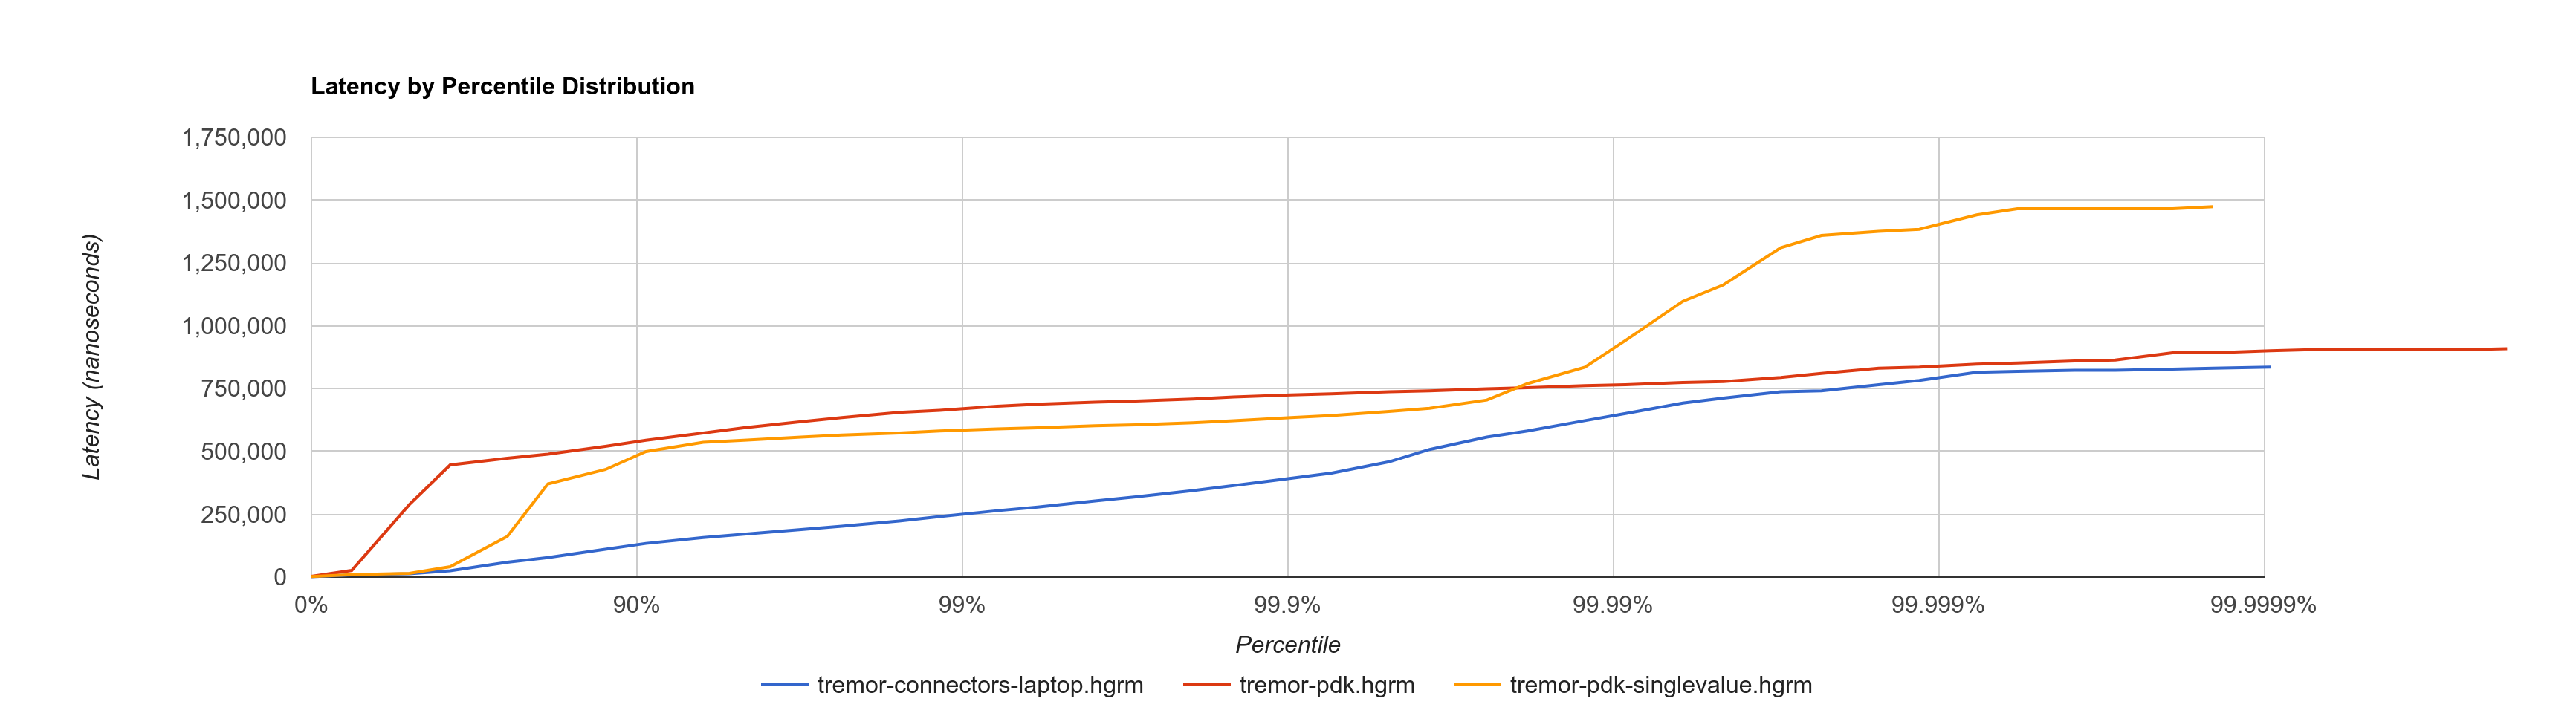
\includegraphics[width=\textwidth]{./Imagenes/histogram_pdk.png}
    \caption{Histograma con dos diferentes versiones del sistema de plugins,
    mejorando la latencia iterativamente. Concretamente, la mejora consiste en
    usar un único \code{Value}, en lugar de la copia \code{PdkValue} (ver
    Anexo~\ref{annex:abi}). La línea marcada como
    \code{tremor-connectors-laptop} es la rama original de Tremor.}%
    \label{fig:histogram_pdk}
\end{sidewaysfigure}

\begin{sidewaysfigure}
    \centering
    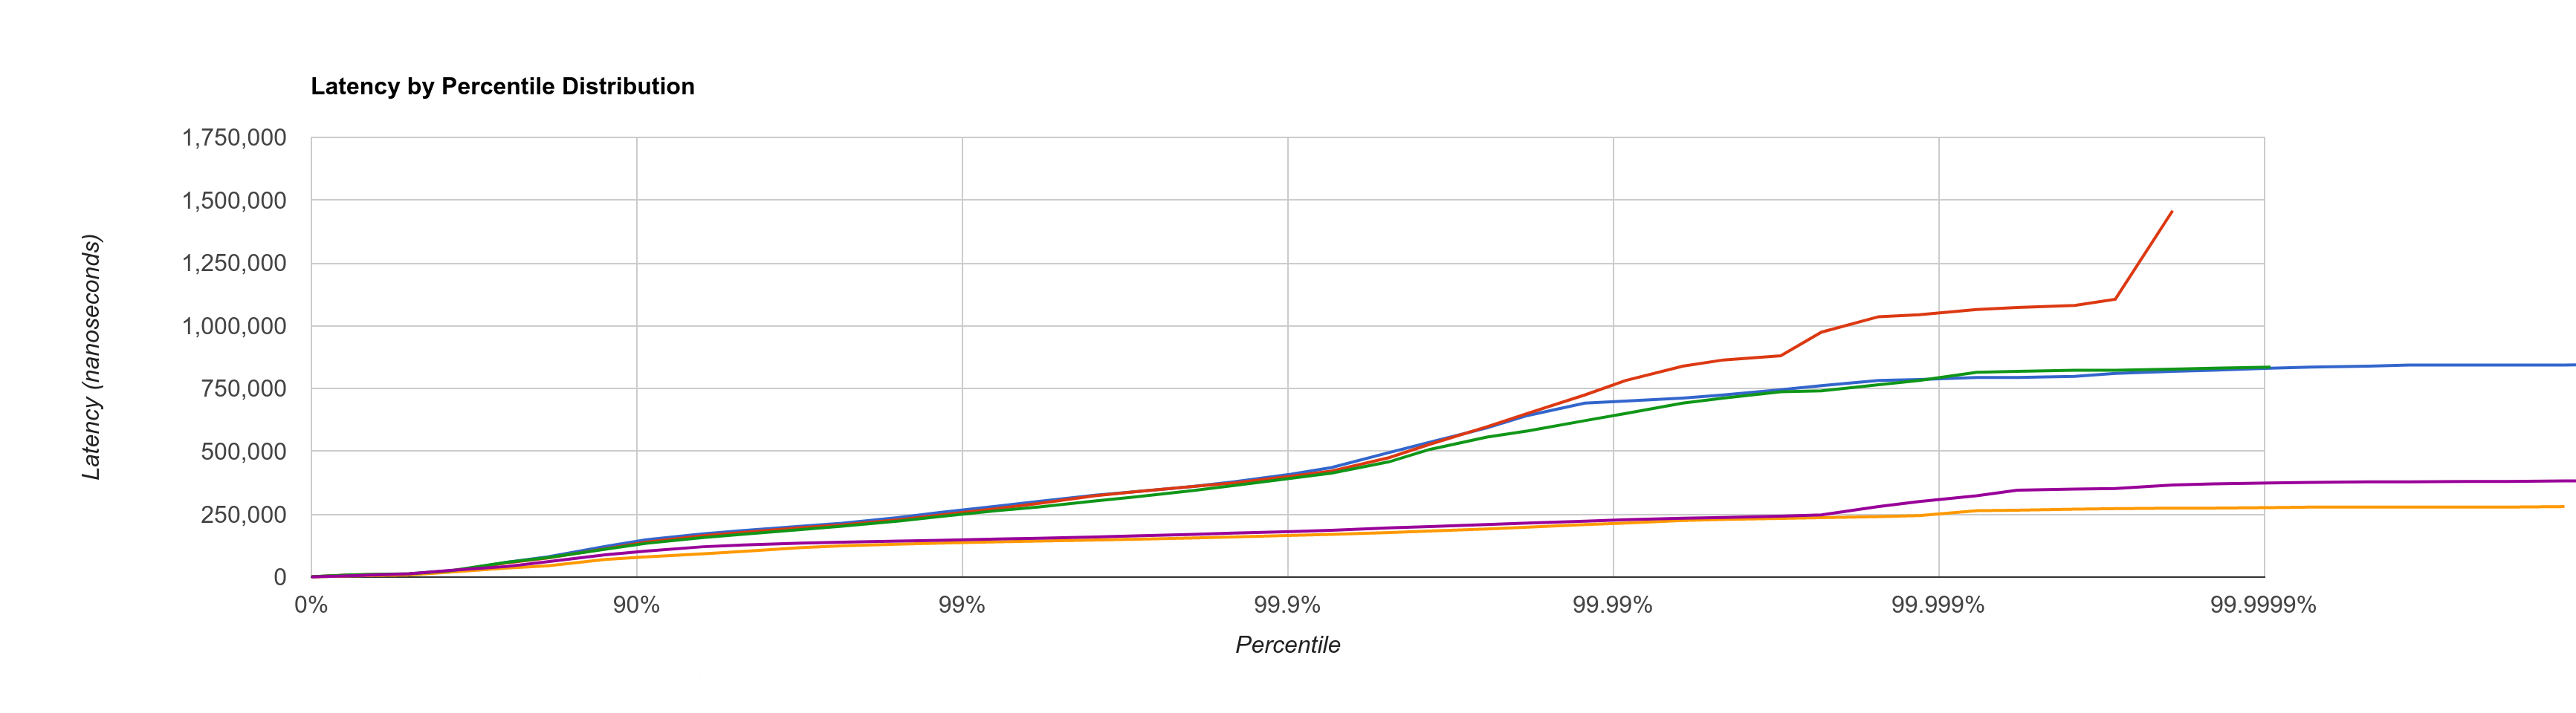
\includegraphics[width=\textwidth]{./Imagenes/histogram_variance.png}
    \caption{Las dos líneas inferiores son el mismo programa ejecutado en el
    servidor dedicado para medir su varianza. Las siguientes dos sobre estas es
    lo mismo con el portátil; la diferencia en varianza no es tan perceptible
    como se esperaba. Una mejora importante en la fiabilidad se consiguió
    realizando varias ejecuciones de calentamiento previas a las mediciones,
    como se puede ver en la diferencia de la línea superior, el portátil sin
    calentamiento, con las otras dos del portátil.}%
    \label{fig:histogram_variance}
\end{sidewaysfigure}

\begin{sidewaysfigure}
    \centering
    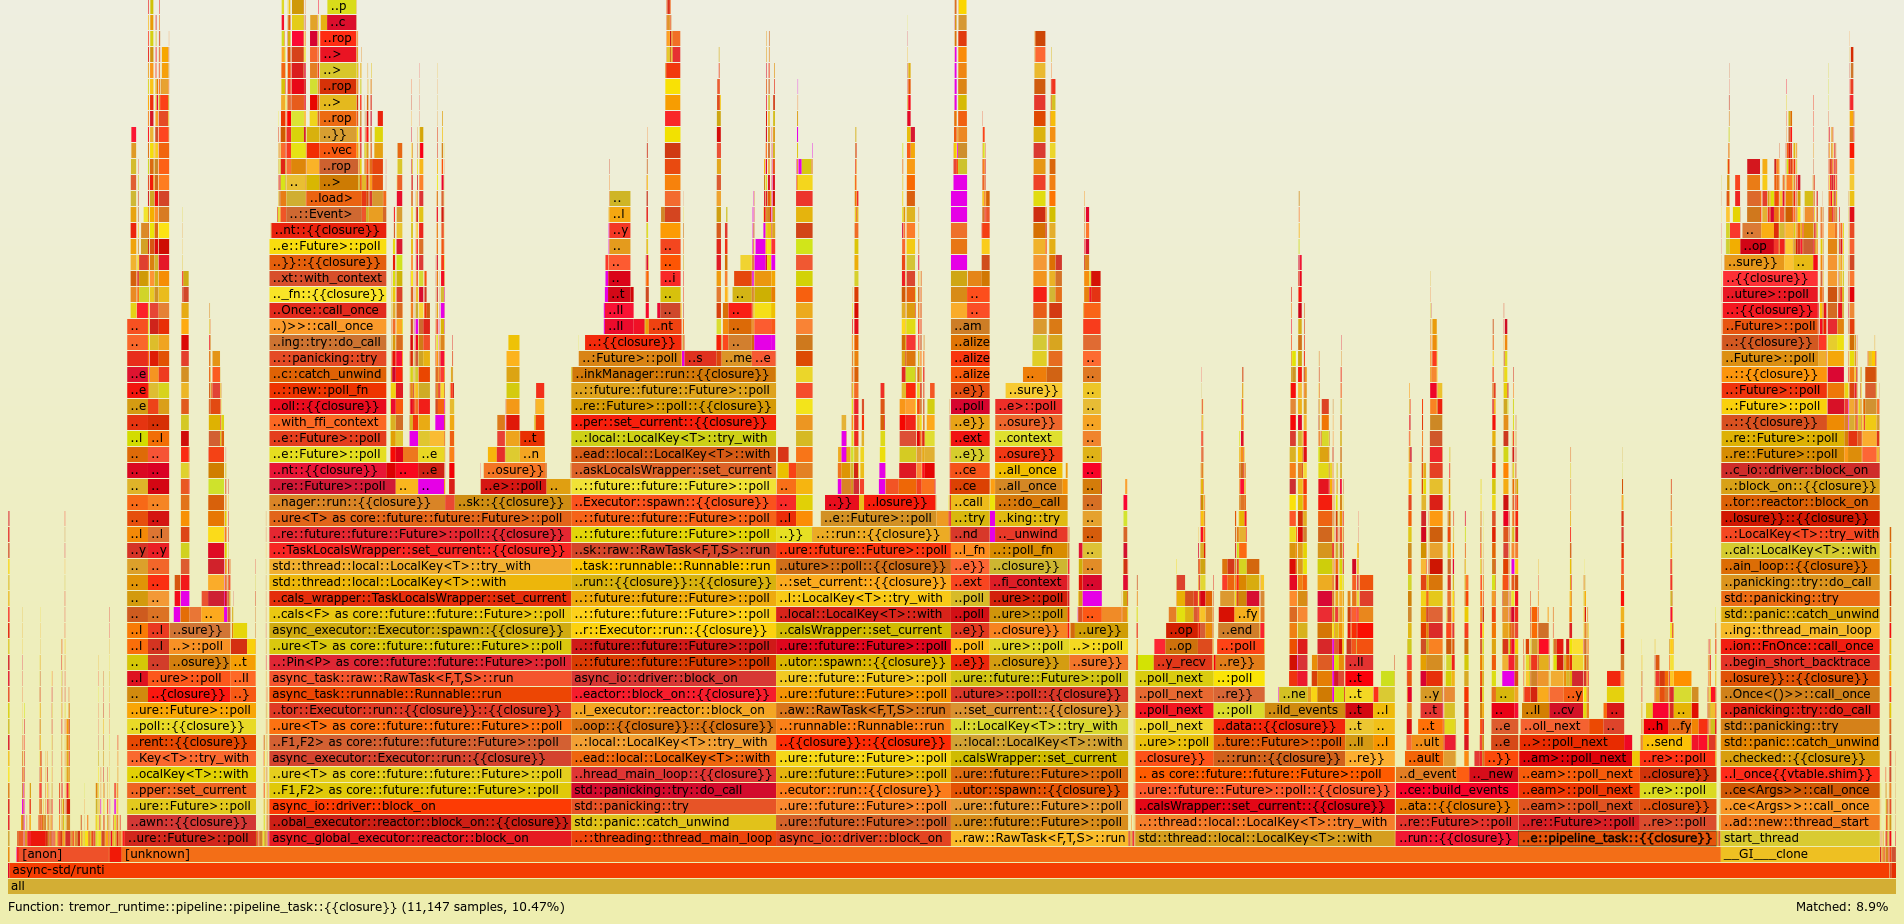
\includegraphics[width=\textwidth]{./Imagenes/without_value_conv.png}
    \caption{\emph{Flamegraph} con los porcentajes de ejecución de Tremor
    original, resaltando en rosa las conversiones de tipos realizadas.}%
    \label{fig:without_value_conv}
\end{sidewaysfigure}

\begin{sidewaysfigure}
    \centering
    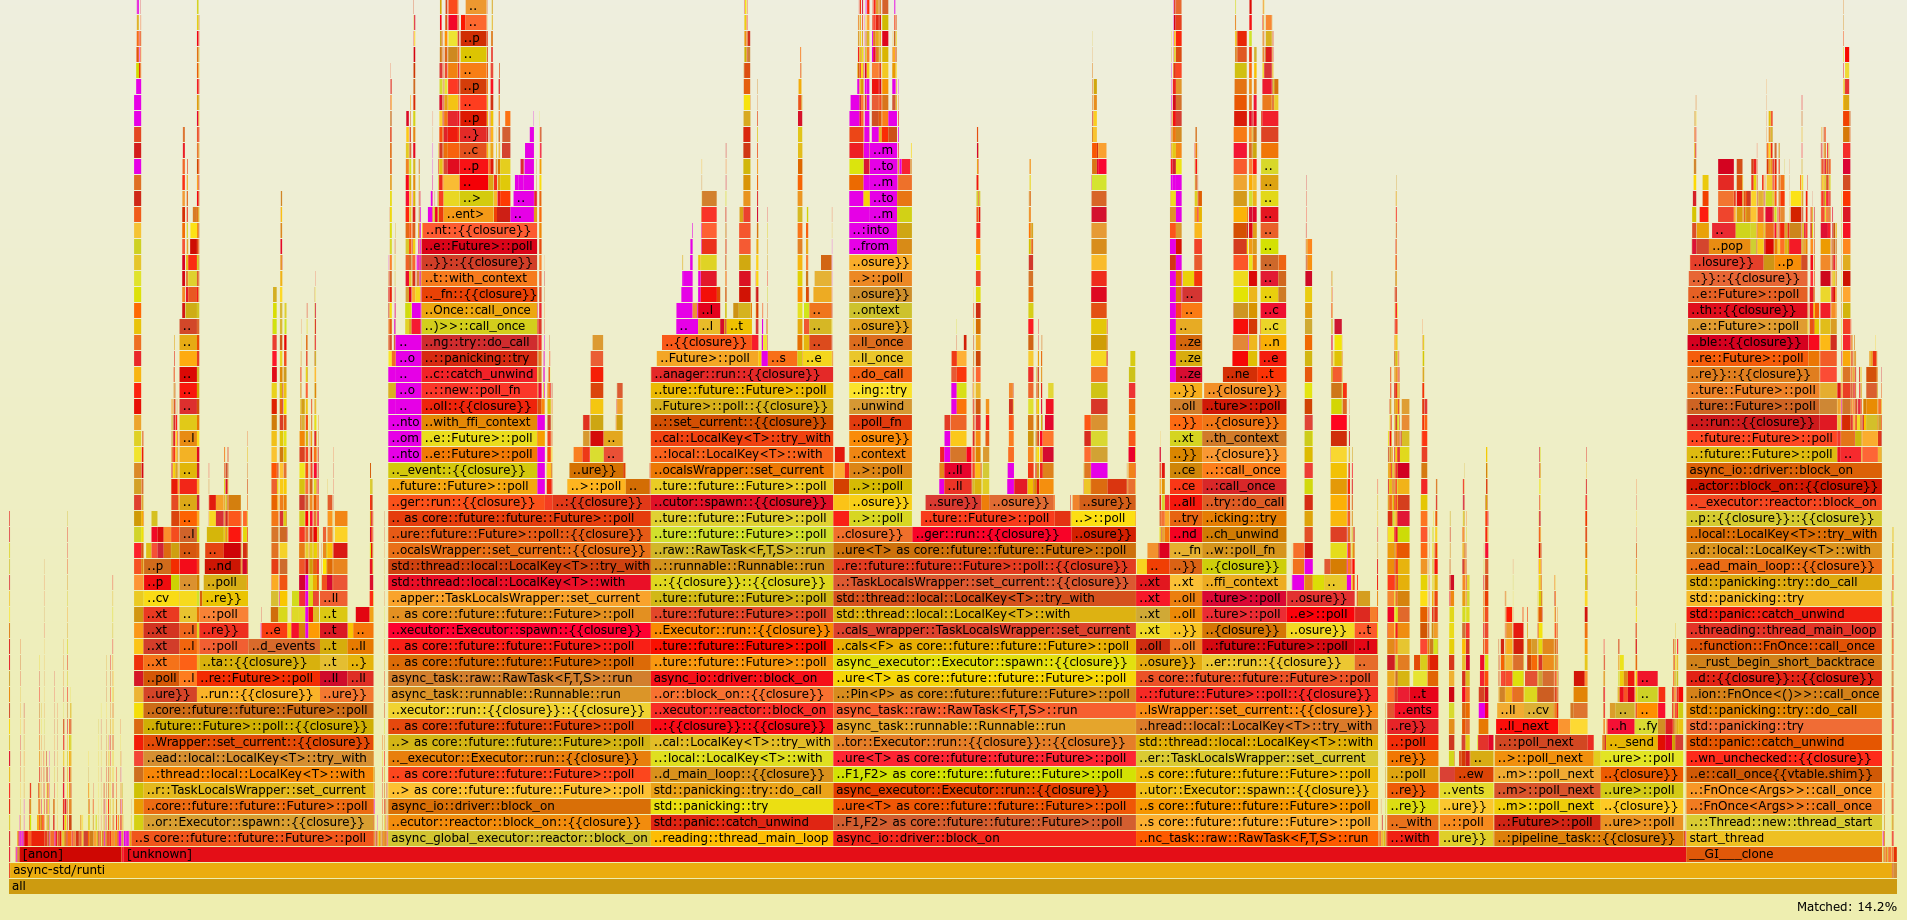
\includegraphics[width=\textwidth]{./Imagenes/with_value_conv.png}
    \caption{\emph{Flamegraph} una vez implementado el sistema de plugins. Las
    conversiones son más visibles ahora, puesto que es necesario para
    comunicarse entre runtime y plugins. Esta gráfica visualiza la degradación
    de rendimiento causada por conversiones de la librería estándar a \abistable
    y viceversa.}%
    \label{fig:with_value_conv}
\end{sidewaysfigure}

\begin{sidewaysfigure}
    \centering
    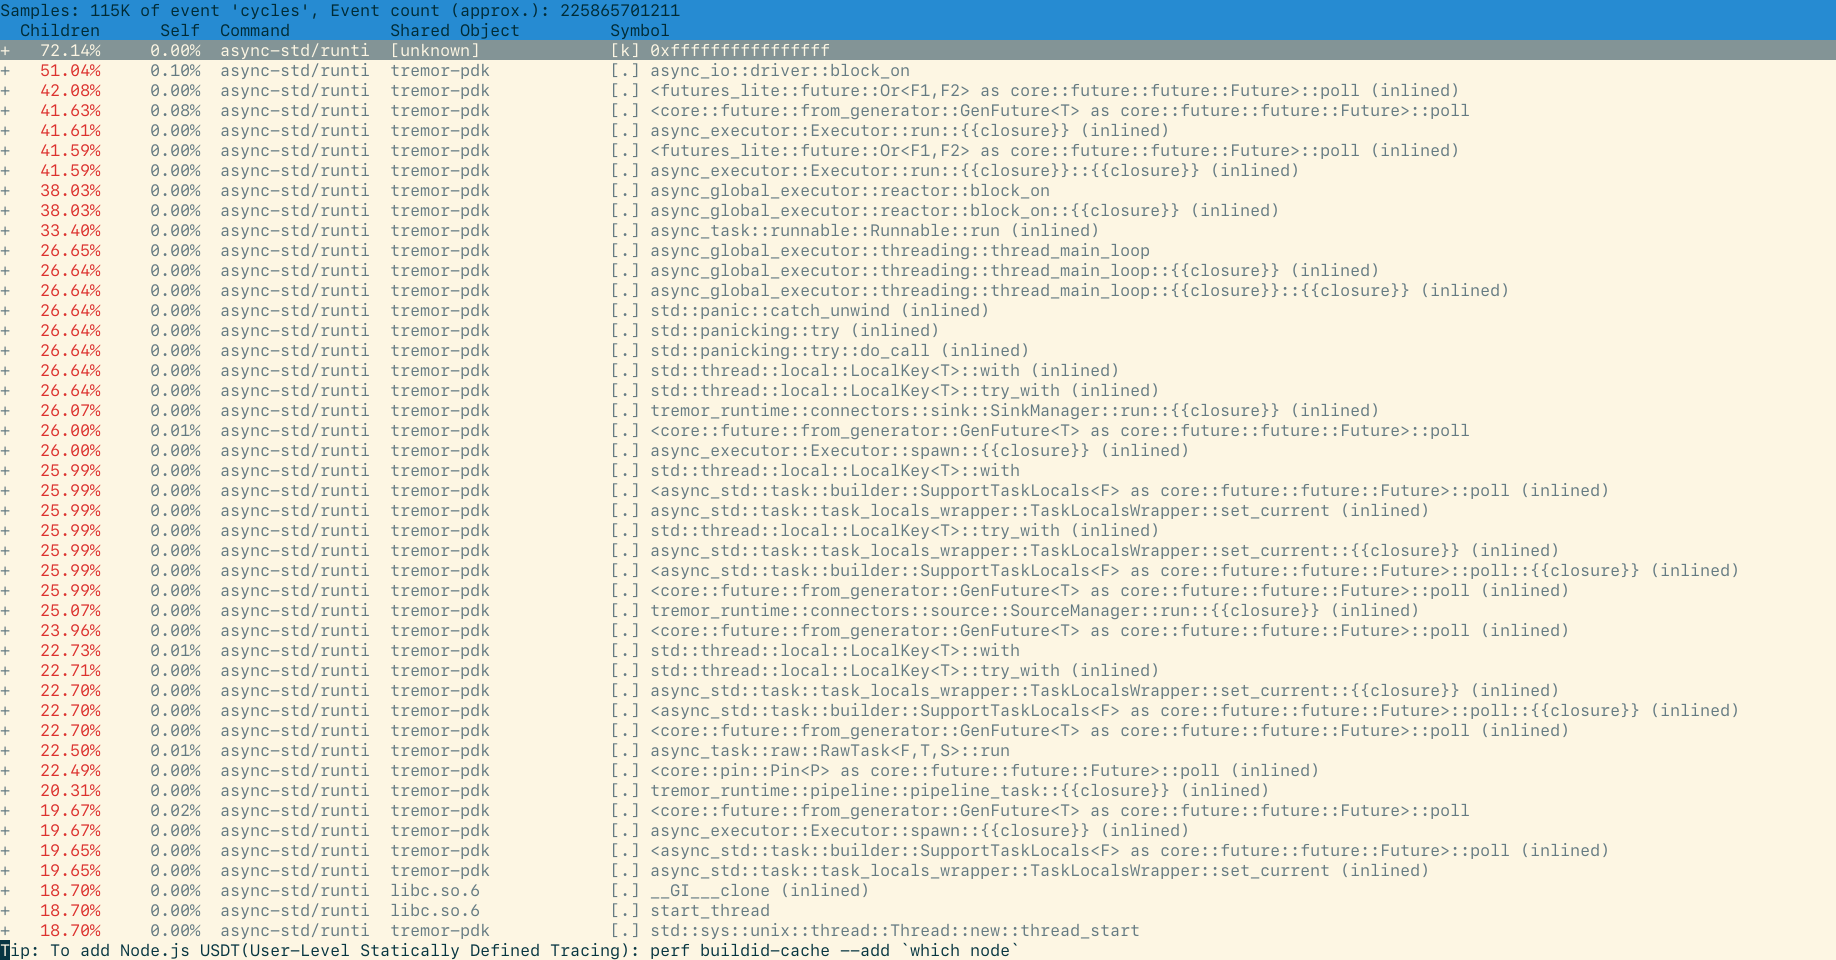
\includegraphics[width=\textwidth]{./Imagenes/perf_report.png}
    \caption{También se utilizó la herramienta \code{perf} para visualizar las
    secciones del programa más frecuentes en su ejecución. El comando completo
    es \code{perf report --no-children -i FILE}. El stack de programación
    asíncrona introduce gran cantidad de ruido, pero sigue pudiéndose distinguir
    por ejemplo \code{SinkManager::run} (ver Anexo~\ref{annex:tremor}), o el uso
    de \code{panic::catch_unwind} para pánicos seguros (ver
    Sección~\ref{sec:panics}).}%
    \label{fig:perf}
\end{sidewaysfigure}

\begin{figure}
    \centering
    \begin{minted}{bash}
#!/usr/bin/env bash

set -e

# Both paths must be absolute, and not use `~` or similars. Otherwise
# it won't work when ran as root.
TREMOR_DIR=/<fill-yours>/tremor-runtime
OUTPUT_DIR=/<fill-yours>/results
WARMUP_ROUNDS=0
BINARIES="tremor-connectors tremor-pdk"
BENCHMARKS="passthrough"

# Working with paths easily
get_dir() {
    dir="$TREMOR_DIR/tremor-cli/tests/bench/$1"
}
get_bin() {
    bin="../../../../target/release/$1"
}

# Validation step to avoid waiting for the benchmarks only for one of
# them to be incorrectly configured.
for bin in flamegraph; do
    if ! command -v "$bin" > /dev/null; then
        echo "ERROR: Binary $bin not available"
        exit 1
    fi
done
for name in $VALUES; do
    get_bin "$name"

    if ! [ -f "$bin" ] || ! [ -x "$bin" ]; then
        echo "ERROR: Binary $bin doesn't exist"
        exit 1
    fi
done
for name in $BENCHMARKS; do
    get_dir "$name"

    if ! [ -d "$dir" ]; then
        echo "ERROR: Benchmark $dir doesn't exist"
        exit 1
    fi
done
echo ">> Verification step passed"

# Setup
mkdir -p "$OUTPUT_DIR"
export TREMOR_PATH=../../../../tremor-script/lib:../../lib/
    \end{minted}
    \caption{Script usado para realizar las pruebas de rendimiento (parte 1/1).}%
    \label{fig:script_bench_1}
\end{figure}

\begin{figure}
    \centering
    \begin{minted}{bash}
# Finally running the benchmarks
for bench in $BENCHMARKS; do
    # Benchmarks only work if you're in the same directory, and then
    # always use relative paths.
    get_dir "$name"
    cd "$dir"

    # Warmup round, ran alternately for accuracy
    for i in $(seq $WARMUP_ROUNDS); do
        for name in $BINARIES; do
            get_bin "$name"

            echo ">> Warming up with $name ($i/$WARMUP_ROUNDS)"
            "$bin" test bench . > /dev/null
        done
    done

    for name in $BINARIES; do
        get_bin "$name"

        echo ">> Benchmarking $name"
        "$bin" test bench . > "$OUTPUT_DIR/${name}.hgrm"

        echo ">> Creating flamegraph for $name"
        flamegraph "$bin" test bench . \
            > "$OUTPUT_DIR/${name}-flamegraph.hgrm"
        mv flamegraph.svg "$OUTPUT_DIR/$name-flamegraph.svg"
        mv perf.data "$OUTPUT_DIR/$name-perf.data"
    done
done
    \end{minted}
    \caption{Script usado para realizar las pruebas de rendimiento (parte 2/2).}%
    \label{fig:script_bench_2}
\end{figure}

\chapter{Fases de desarrollo}\label{annex:hours}

Este anexo lista las fases en las que se llevó a cabo el proyecto y las horas
invertidas en cada una de ellas. Se incluye el periodo en el que se realizaron,
comenzando en abril de 2021 con la propuesta a Tremor. Una vez aceptado, el
inicio oficial se dio en agosto. Adicionalmente, junto a sus descripciones se
añaden uno o más enlaces relacionados con la tarea.

\setlist{topsep=2pt,nosep}

\begin{longtable}[H]{| m{9.7cm} | P{1.3cm} | P{3.4cm} |}
\caption{Fases de desarrollo del proyecto}\\

\hline
\textbf{Fase}
    & \textbf{Horas}
    & \textbf{Periodo} \\
\hline
\endhead

Propuesta a Tremor: incluye una introducción sobre quién soy, qué proyecto
quiero hacer y una breve planificación de la metodología a seguir.

\vspace{4mm}
\emph{\url{https://nullderef.com/blog/gsoc-proposal/}}
    & 6
    & Abr.~\textquotesingle21 \\

\hline
Investigación inicial de las tecnologías disponibles para el sistema de
plugins y discusión con el equipo. Esto también formó parte de la propuesta,
aunque de forma no oficial.

\vspace{4mm}
\emph{\url{https://nullderef.com/blog/plugin-tech/}}
    & 36
    & Abr.~\textquotesingle21 -- May.~\textquotesingle21 \\

\hline
Aceptación del proyecto. Introducción a Tremor y a su equipo.

\vspace{4mm}
\emph{\url{https://nullderef.com/blog/plugin-start/}}
    & 8
    & Ago.~\textquotesingle21 \\

\hline
Implementación de prototipos para el sistema de plugins, y medidas de
rendimiento iniciales. También incluye otros experimentos menores para encontrar
el mejor método para tener programación asíncrona o genéricos.

\vspace{4mm}
\emph{\url{https://github.com/marioortizmanero/pdk-experiments}}

\vspace{4mm}
\emph{\url{https://nullderef.com/blog/plugin-start/}}

\vspace{4mm}
\emph{\url{https://nullderef.com/blog/plugin-dynload/}}
    & 51
    & Ago.~\textquotesingle21 -- Feb.~\textquotesingle22 \\

\hline
Investigación del funcionamiento interno de Tremor. Diseño de diagramas de
secuencia.

\vspace{4mm}
\emph{\url{https://nullderef.com/blog/plugin-dynload/}}
    & 13
    & Sep.~\textquotesingle21 \\

\hline
Investigación en detalle de cargado dinámico en Rust.

\vspace{4mm}
\emph{\url{https://nullderef.com/blog/plugin-dynload/}}
    & 22
    & Sep.\textquotesingle21 -- Oct.~\textquotesingle21 \\

\hline
Aprendizaje de la librería \abistable.

\vspace{4mm}
\emph{\url{https://nullderef.com/blog/plugin-abi-stable/}}
    & 17
    & Oct.~\textquotesingle21 -- Nov.~\textquotesingle21 \\

\hline
Soporte de \abistable para programación asíncrona con \code{async_ffi}.

\vspace{4mm}
\emph{\url{https://github.com/oxalica/async-ffi/pull/10}}
    & 15
    & Nov.~\textquotesingle21 -- Ene.~\textquotesingle22 \\

\hline
Primer diseño e implementación del sistema de plugins.

\vspace{4mm}
\emph{\url{https://github.com/tremor-rs/tremor-runtime/pull/1434}}
    & 64
    & Oct.~\textquotesingle21 -- Abr.~\textquotesingle22 \\

\hline
Mediciones de rendimiento.

\vspace{4mm}
\emph{\url{https://github.com/marioortizmanero/nullderef.com/pull/54} (artículo
aún no publicado)}
    & 14
    & Ene.~\textquotesingle22 -- Jun.~\textquotesingle22 \\

\hline
Resolución de los problemas de covarianza y subtipado.

\vspace{4mm}
\emph{\url{https://github.com/rodrimati1992/abi_stable_crates/issues/75}}
    & 26
    & Ene.~\textquotesingle22 -- Mar.~\textquotesingle22\\

\hline
Añadir soporte de la librería \code{halfbrown} para \abistable.

\vspace{4mm}
\emph{\url{https://github.com/rodrimati1992/abi_stable_crates/pull/83}}
    & 19
    & Mar.~\textquotesingle22 -- Jun.~\textquotesingle22 \\

\hline
Segunda versión del sistema de plugins con las dos mejoras anteriores de
rendimiento.

\vspace{4mm}
\emph{\url{https://github.com/tremor-rs/tremor-runtime/pull/1597}}
    & 26
    & May.~\textquotesingle22 -- Jun.~\textquotesingle22 \\

\hline
Documentación final para que Tremor pueda continuar con el desarrollo del
proyecto.

\vspace{4mm}
\emph{\url{https://github.com/tremor-rs/tremor-runtime/pull/1597}}

\vspace{4mm}
\emph{\url{https://github.com/marioortizmanero/tremor-runtime/projects/1}}
    & 6
    & Jun.~\textquotesingle22 \\

\hline
Memoria del Trabajo de Fin de Grado.
    & 54
    & May.~\textquotesingle22 -- Jun.~\textquotesingle22 \\

\hline
\textbf{Total}
    & \textbf{379}
    & \textbf{Abr.~\textquotesingle21 --
Jun.~\textquotesingle22} \\

\hline
\end{longtable}


\end{document}
